% MSc dissertation example file, February 2022
%
% Leave one of the documentclass lines uncommented to match your degree.
% You may remove the logo option if it causes problems.
% Do not change any other options.
% \documentclass[logo,msc,adi]{infthesis}     % Adv Design Inf
% \documentclass[logo,msc,ai]{infthesis}      % AI
% \documentclass[logo,msc,cogsci]{infthesis}  % Cognitive Sci
\documentclass[logo,msc,cs]{infthesis}      % Computer Sci
% \documentclass[logo,msc,cyber]{infthesis}   % Cyber Sec
% \documentclass[logo,msc,datasci]{infthesis} % Data Sci
% \documentclass[logo,msc,di]{infthesis}      % Design Inf
% \documentclass[logo,msc,dsti]{infthesis}    % Data Sci TI
% \documentclass[logo,msc,inf]{infthesis}     % Informatics
% \documentclass[logo,msc]{infthesis}           % degree unspecified, do not change except to add your degree
%%%%%%%%%%%%%%%%%%%%%%%%
% Understand any problems and seek approval before assuming it's ok to remove ugcheck.
\usepackage{msccheck}

% Include any packages you need below, but don't include any that change the page
% layout or style of the dissertation. By including the ugcheck package above,
% you should catch most accidental changes of page layout though.

\usepackage{microtype} % recommended, but you can remove if it causes problems

\usepackage{tabularx}
\usepackage{makecell}
\usepackage{graphicx}
\usepackage{hyperref}

\begin{document}
\begin{preliminary}

\title{Design and Implementation of a Resource-based Checklist Generation Tool}

\author{Watcharin 'Aun' Sirinaovakul}

\date{\today}

\abstract{
% This skeleton demonstrates how to use the \texttt{infthesis} style for
% MSc dissertations in the School of Informatics. It also emphasises the
% page limit and associated style restrictions for Informatics dissertations
% with course code \texttt{INFR11077}. If your degree has a different project
% course code, then it is likely to have different formatting rules.
% The file \texttt{skeleton.tex} generates this document and should be used as a
% starting point for your thesis. Replace this abstract text with a concise
% summary of your report.

% what I did, evaluation
}

\maketitle

\newenvironment{ethics}
   {\begin{frontenv}{Research Ethics Approval}{\LARGE}}
   {\end{frontenv}\newpage}

\begin{ethics}
% IF ETHICS APPROVAL WAS REQUIRED:
This project obtained approval from the Informatics Research Ethics committee.\\
Ethics application number: 486463\\
Date when approval was obtained: 2022-06-30

\standarddeclaration
\end{ethics}


\begin{acknowledgements}
Any acknowledgements go here.
\end{acknowledgements}


\tableofcontents
\end{preliminary}


\chapter{Introduction}
% objective, users, benefits, scope of work, relevant works, previous works, future works, project background, techniques

% The preliminary material of your report should contain:
% \begin{itemize}
% \item
% The title page.
% \item
% An abstract page.
% \item
% Declaration of ethics and own work.
% \item
% Optionally an acknowledgements page.
% \item
% The table of contents.
% \end{itemize}

% As in this example \texttt{skeleton.tex}, the above material should be
% included between:
% \begin{verbatim}
% \begin{preliminary}
%     ...
% \end{preliminary}
% \end{verbatim}
% This style file uses roman numeral page numbers for the preliminary material.

% The main content of the dissertation, starting with the first chapter,
% starts with page~1. \emph{\textbf{The main content must not go beyond page~40.}}

% The report then contains a bibliography and any appendices, which may go beyond
% page~40. The appendices are only for any supporting material that's important to
% go on record. However, you cannot assume markers of dissertations will read them.

% You may not change the dissertation format (e.g., reduce the font size, change
% the margins, or reduce the line spacing from the default 1.5 spacing). Be
% careful if you copy-paste packages into your document preamble from elsewhere.
% Some \LaTeX{} packages, such as \texttt{fullpage} or \texttt{savetrees}, change
% the margins of your document. Do not include them!

% Over-length or incorrectly-formatted dissertations will not be accepted and you
% would have to modify your dissertation and resubmit. You cannot assume we will
% check your submission before the final deadline and if it requires resubmission
% after the deadline to conform to the page and style requirements you will be
% subject to the usual late penalties based on your final submission time.

% \section{Using Sections}

% Divide your chapters into sub-parts as appropriate.

% \section{Citations}

% Citations (such as \cite{P1} or \cite{P2}) can be generated using
% \texttt{BibTeX}. For more advanced usage, we recommend using the \texttt{natbib}
% package or the newer \texttt{biblatex} system.

% These examples use a numerical citation style. You may use any consistent
% reference style that you prefer, including ``(Author, Year)'' citations.


% objective, users, benefits, scope of work, relevant works, previous works, future works, project background, techniques

-Probably what a workflow is-

Business process management (BPM) tools are software to help design, automate, and manage systematic workflows for various business areas. The ease with which repetitive task automation can be implemented using BPM tools is one of its primary benefits. That is because it requires no prior coding experience to develop a workflow in BPM tools. However, the tools are sufficiently customisable for a more experienced user to create a more complex workflow.

% WorkflowFM \cite{papapanagiotou2017workflowfm} is a BPM tool developed and maintained by a research team at the University of Edinburgh that allows people in various industries to build their automated workflows from scratch. What distinguishes WorkflowFM from other competitors is that the models are based on the data structure of the input and output of each task. This further reduces the complexity when generating codes since the system can rely on the structure of the resources rather than the arbitrary input and output defined by users. Moreover, WorkflowFM can generate code required for the control flow automatically. Despite the advantages provided by WorkflowFM, it is still in a very early stage with limited features.

WorkflowFM \cite{papapanagiotou2017workflowfm} is a BPM tool developed by a research team at the University of Edinburgh.
% WorkflowFM's main goal is to help create workflows strictly to the data models within the system. That means each process needs to strictly follow the data models provided within the system and no arbitrary information are allowed.
The objective of WorkflowFM is to assist in developing workflows that rigorously adhere to the system's data models. This means that no random information is permitted and that each process must strictly follow to the data models supplied within the system.
% Compared to other competitors which do not rigorously conform to the data models, WorkflowFM is easier to ge
Nevertheless, WorkflowFM is still in a very early stage with limited features.

-Probably what a checklist is and why it is important-

-What I am going to do in this project-

-What scope of the project I am looking to do-

-What end results of the project should look like-


\chapter{Background}

\section{Business Process Management Tools}
% Business Process Management (BPM) is a methodology that involves designing, controlling, and analysing business processes to support organisations \cite{bpmdefinition}. 
% BPM's stages is defined differently depending on references \cite{bpmlifecycles, bpmlifecycles2, bpmlifecycles3}; however, it generally consists of at least four stages: i) analysing; ii) modeling; iii) implementing; iv) executing.
% As for BPM tools, they are software solutions that support organisations in all stages of BPM with little to no coding knowledge. As a consequence, BPM tools are widely used in various industries.
Business Process Management (BPM) is a discipline that assist business analysts in planning, monitoring and analysing processes to support businesses \cite{bpmdefinition}. BPM methodologies could generally be separated into four different stages: i) analysing; ii) modelling; iii) implementing; iv) execution \cite{bpmlifecycles, bpmlifecycles3, bpmlifecycles2}.
BPM tools are software that makes use of this concept in assisting business analysts model processes with little to no coding knowledge to help businesses build automatic streamlining and reduce wastes in manufacturing processes 
\cite{bpmtoolwaste}.

One of the advantages of using BPM tools is the orchestration between systems, humans, and workflows \cite{bpmstrength}.
This improves the efficiency of business processes in organisations by formalising processing into structured methods that can be monitored, analysed, and automated easily \cite{bpmbenefits}.
BPM tools use checklists that are integrated as part of a workflow to efficiently coordinate humans and workflows by integrating inputs into the workflow. For example, Bizagi \cite{bizagi}, one of the widely known BPM tools, can construct checklists or forms within its automated workflows and connect the checklists to the following processes using the shared database technique. Nintex \cite{nintext} is another widely used BPM tool that also adopts the idea of checklist and implements it in their environment. This provides a variety of options for workflow users to interact with the workflows in the system.


\section{WorkflowFM}
\label{background:workflowfm}

WorkflowFM \cite{papapanagiotou2017workflowfm} is a logic-based BPM tool developed by researchers from the University of Edinburgh. Being a logic-based framework means all the inputs, outputs, and processes follow the validation defined by the framework.
Each process is validated by WorkflowFM to ensure that it is logically valid, correctly matched with neighbour processes, and functional as a workflow.
As a logic-based BPM tool, WorkflowFM differs from other frameworks in that processes are defined based on inputs and outputs with preconditions, as opposed to most BPM tools which accept any Business Process Model and Notation (BPMN) \cite{bpmn} format when creating a workflow. Moreover, it requires the inputs and outputs in each process to match when connected to other processes.
% Additionally, WorkflowFM requires defining data models for each input and output
% only require a XML pattern to create a workflow as XML is the standardised format for BPM tools.
% unlike various BPM tools which follows the XML Process Definition Language (XPDL), the standard format for interchanging process definitions between different BPM tools \cite{xmlpdl}.



WorkflowFM's system architecture, as shown in Figure \ref{fig:workflowfm-system}, includes two main groups of components: modelling and execution. Modelling is the part that allows users to create workflows, and execution is the component that operates deployed workflows in the system. This project aims to build a checklist generation tool as an extension to the execution engine to help generate checklists in WorkflowFM and allow people to perform tasks through checklists for executing workflow processes.


% , which contains two components: composer and reasoner. The composer component assists users in creating workflows, while the reasoner validates that the workflows produced by the composer adhere to the defined inputs and outputs.
% On the other hand, m and contains three components: execution engine, simulation engine, and dashboard.
% The checklist generation will be placing in the execution group as an extension to the execution engine.

% WorkflowFM's system architecture, as shown in Figure \ref{fig:workflowfm-system}, includes two main groups of components: modelling and execution. Modelling is the part that allows users to create workflows, which contains two components: composer and reasoner. The composer component assists users in creating workflows, and the reasoner validates that the workflows produced by the composer adhere to the defined inputs and outputs.
% On the other hand, execution is the component that operates deployed workflows in the system. Execution contains execution engine, simulation engine, and dashboard.
% This project aimed to build was a checklist generation tool that connects with the execution engine as an extension to generate checklists and allow people to perform tasks for executing workflow processes.
% The execution engine and the simulation engine are integrated with each other and directly connect to the dashboard to visualise deployed workflows. Furthermore, the checklist generation connects with the execution engine as an extension to generate checklists and allow people to perform tasks for workflows.
% Unlike Bizagi or Nintex, WorkflowFM is a logic-based framework which 

\begin{figure}
    \centering
    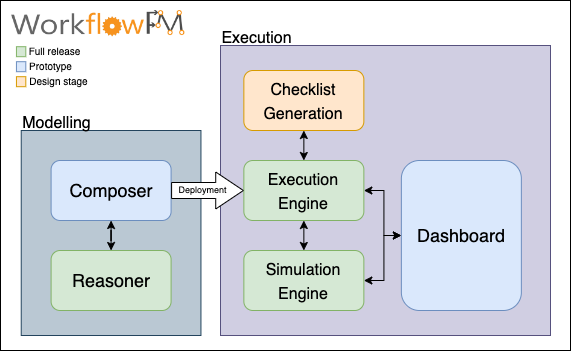
\includegraphics[width=0.7\textwidth]{overleaf/images/workflowfm-system.png}
    \caption{WorkflowFM's System Architecture}
    \label{fig:workflowfm-system}
\end{figure}

As of now, WorkflowFM has been used in the healthcare and manufacturing domains. With the expanding usage of the framework, the checklist generation becomes more desirable for people in the industries. However, checklist generation is still at the design stage and has not been implemented. That is why this project focuses on implementing a prototype of the checklist generation.

% As of now, WorkflowFM has been used in the healthcare domain \cite{papapanagiotou2014formal} and expanding to the manufacturing domain. With in increasing of ..., this is why a checklist generation tool is needed in WorkflowFM.

\section{WorkflowFM's Process}
\label{background:input_output}

Each process in WorkflowFM contains a unique name and a group of inputs and a group of outputs. Each input and output is represented as a node that can be either atomic, parallel, or optional. 
An atomic is a representation of an entity \cite{entity} that exists in the system,
a parallel is a representation of selecting every children node,
and an optional is a representation of selecting one among all the children nodes.
Combining the nodes together would form a tree of nodes, which a leaf node must be an atomic.

For example, according to the running example in Section \ref{running_example}, the process's name is \verb!Payment Process!, the input contains an optional node that can be either an order (\verb!order!) or an order with discounts (\verb!order with discounts!), and the output contains a parallel node of the billing address (\verb!billing address!) and an optional node that can be either PayPal (\verb!paypal!) or Debit/Credit card (\verb!debit/credit card!). A visualisation of the inputs and outputs can be visualised in Figure \ref{fig:type_nodes_example}.

\begin{figure}[ht!]
    \centering
    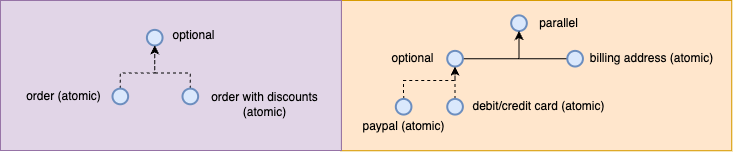
\includegraphics[width=\textwidth]{overleaf/images/type_nodes_example.png}
    \caption{Inputs (Left) and Outputs (Right) Visualisation}
    \label{fig:type_nodes_example}
\end{figure}


% A JSON-based format \cite{json} is used in WorkflowFM to specify processes.
% The JSON format used in WorkflowFM includes several fields that are used in different parts of the system, which can be seen in Figure \ref{fig:workflowfm_json}.
% However, the name, input and output of each process are the only requirements to generate a resource-based checklist template.
% % Each model consists of \verb!type!, \verb!name!, and \verb!args!. There are only three types in \verb!type!: \verb!var!, \verb!plus!, and \verb!times!. 

% \begin{figure}[ht!]
%     \centering
%     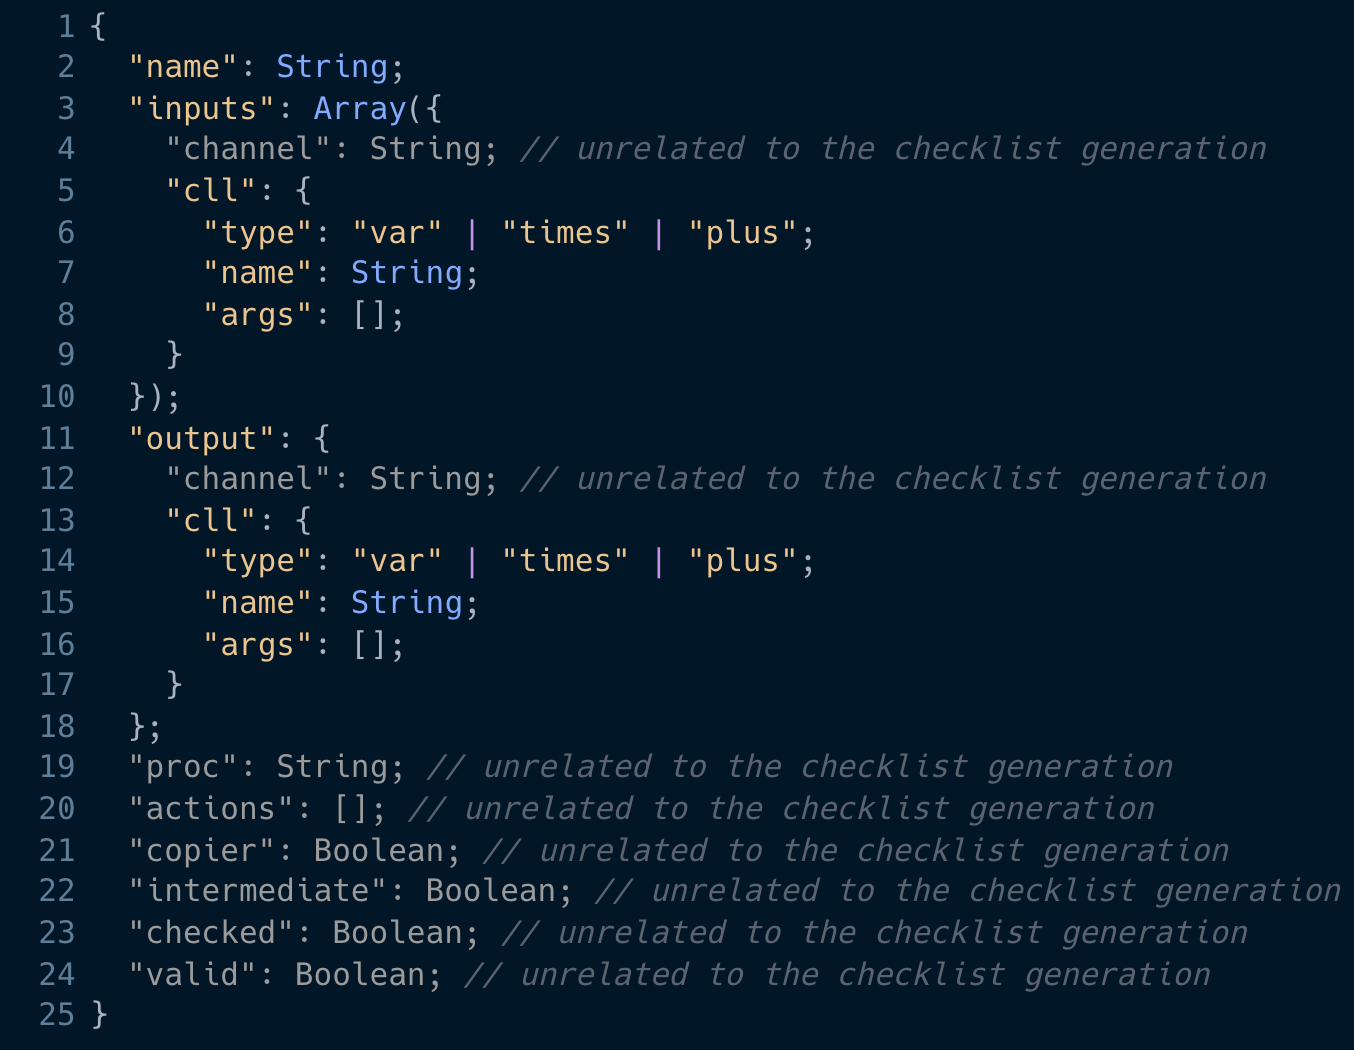
\includegraphics[width=0.75\textwidth]{overleaf/images/workflowfm_json.png}
%     \caption{WorkflowFM's Process JSON}
%     \label{fig:workflowfm_json}
% \end{figure}


% Each input and output node can only be in one of the three types including \verb!var!, \verb!times!, and \verb!plus!.
% A \verb!var! node is a terminal node. That means a \verb!var! node must have no child. Being a \verb!var! node indicates that that specific node is a data model that the process can refer to.
% On the other hand, \verb!times! and \verb!plus! nodes are not data models on its own and must contain child nodes inside it. The child nodes can either be one of the three types recursively, but at terminal nodes, they must be the \verb!var! type.
% \verb!times! and \verb!plus! nodes are different on how they combine the children. \verb!times! merges all the children together as one large data model, while \verb!plus! only selects one of its children to be the data model representing that node.

% All child nodes under \verb!times! are required to exist as the data model representing that node, while only one of the children under \verb!plus! is the representative data model. 

% but they must contain nodes as their children. The difference between \verb!times! and \verb!plus! is all child nodes in a \verb!times! node are compulsory inputs or outputs, while a \verb!plus! node needs only one of the child nodes to be an input or output.

% A process contains nodes from both input and output sides. A node is a representation between three things: a data model, a times operator, and a plus operator. A data model will be referred as the \verb!var! type. A times operator and a plus operator will be referred as \verb!times! and \verb!plus! accordingly. Both \verb!times! and \verb!plus! nodes must contain children since they are not data models. Furthermore, their children can either be \verb!var!, \verb!times!, and \verb!plus!. However, if a child node is either \verb!times! or \verb!plus!, it needs to recursively continue having children. A \verb!var! child, however, contains no children and acts as a terminal node. \verb!times! and \verb!plus! are different on how they operate. \verb!times! combines the children together as one large data model, while \verb!plus! only selects one of its children to be the data model representing that node.

% The input and output of a process are represented as nodes. A node can either be an atomic entity (\verb!var!) \cite{entity} or an operator (\verb!times! or \verb!plus!).
% An atomic entity represents an entity in the system's database.
% An operation which combines multiple nodes is called a times operator, while which selects an entity between a group of nodes is called a plus operator.
% Combining both entities and operators would form into a tree of nodes, which a leaf node of this tree must be an entity.

% For example, in Figure \ref{fig:process_flows} | which has the JSON format provided in Appendix \ref{appendix:fig:example_json}, this is a payment process that receives \verb!orders! and \verb!payment_method! as the input and returns \verb!order_receipt! and either \verb!credit_card_receipt! or \verb!change! as the output depending on what \verb!payment_method! coming in.
% All five of them are terminal nodes and data models of this process. On the input part, both \verb!orders! and \verb!payment_method! are connected to a \verb!times! node indicating that both data models are compulsory. Meanwhile, \verb!credit_card_receipt! and \verb!change! are connected to a \verb!plus! node indicating either one between them can be selected as the representing data model; however, not both. On top of that, the \verb!plus! node is connected to a \verb!times! node along with \verb!order_receipt! indicating both of them are compulsory.

% Ultimately, the input of this payment process is ``\verb!orders! and \verb!payment_method!"; and the output of this payment process is either ``\verb!order_receipt! and \verb!change!" or ``\verb!order_receipt! and \verb!credit_card_receipt!".

% the input node is a \verb!plus! and contains two children: \verb!input_var_node_1! and \verb!input_times_node!. Moreover, one of the children is a \verb!times! and contains two children: \verb!input_var_node_2! and \verb!input_var_node_3!. Ultimately, the input of this process can be either:

% \begin{itemize}
%     \item \verb!input_var_node_1! \vspace{-8px}
%     \item (\verb!input_var_node_2!, \verb!input_var_node_3!)
% \end{itemize}

% The output of the process is less complex in comparison to the input.
% The output node is a \verb!times! and has only two \verb!var! children. This makes (\verb!output_var_node_1!, \verb!output_var_node_2!) as the output of this process.

% That means either \verb!input_var_node_1! or \verb!input_var_node_2! can be the input data model of the process. Meanwhile, the output node is \verb!times! and also contains two children. In contrast to \verb!plus!, \verb!output_var_node_1! and \verb!output_var_node_2! are the output data models of the process.

% \begin{figure}[ht!]
%     \centering
%     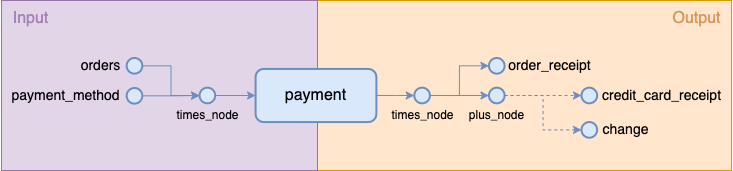
\includegraphics[width=\textwidth]{overleaf/images/process_flows.png}
%     \caption{Example Process}
%     \label{fig:process_flows}
% \end{figure}

\section{Generation of structured checklists from formal \\resource-based workflow models}
\label{background:chens_design}
% This is an MSc project from the previous year written by Yefei Chen \cite{checklistdesign}. Chen has designed the user interface for WorkflowFM's checklist generation tool as well as solved some of the theoretical challenges in the design, such as function-flow chart and data model design. Chen's design consists of six features: i) main page; ii) canvas; iii) edit checklist dependencies; iv) process checklist; v) finished checklist; vi) design of checklist. In the end, the system usability scale questionnaire (SUS) score was mediocre, with a score of 56.5. However, Chen discussed the design weaknesses and provided an analysis of them. Consequently, the results are extremely important since we could continue improving the design based on the analysis.

A design of a resource-based checklist generator has been proposed in Yefei Chen's MSc dissertation \cite{checklistdesign}.
Chen's design is based on the fact that WorkflowFM contains all the data models of the workflow processes in the system and utilises this fact by allowing the checklist generation tool being able to link dependencies with the checklist, which will be further explained in Section \ref{background:dependencies}. This is the feature that we adopted into our project.

Although our project was building on top of Chen's design, Chen's design could not be used to 


\section{Dependencies}

\section{Data Models}


% The design consists of four user interfaces with functionalities on each screen as follow:

% \begin{itemize}
%     \item \textbf{Main Page} is the landing screen of the checklist generator. It can be divided into three sections: \verb!Start A Checklist!, \verb!In Progress!, and \verb!Finished!. The \verb!Start A Checklist! section will bring the user to Canvas screen to create a template. The \verb!In Progress! section is the section that contains all the checklists that has already been started, but not yet finished. And lastly, the \verb!Finished! section contains all the finished checklists.
%     \item \textbf{Canvas} is the building templates screen. It allows users to custom the title, question names, types, and other things in checklists.
%     \item \textbf{Edit Checklist Dependencies} is the screen to manage dependencies in a template. Once a template has been created in Canvas, the designer sometimes needs to adjust dependencies between the input and output. That is to allow the system to create connections between components.
%     \item \textbf{Process Checklist} is the screen of a finished template. It displays the information according to the designed template in Canvas. A finished template, or checklist, in this screen will be used to perform tasks for workflow processes in WorkflowFM.
% \end{itemize}



% \chapter{Methodology}
% % overall design, architectural design, interface design, database design
% % implementation - frontend (main, canvas, checklist) and backend (template creation, template storing, 3, 4)
% % user diagram
% To accomplish the objectives of this project, we separated them into major milestones and had a weekly meeting with the supervisor to update our progress and see how the schedule went according to the initial plan. In the end, we ended up having four different stages to develop this project: design, implementation, testing, and evaluation.

\section{Design}
Before the design stage, we started gathering and analysing requirements from multiple sources including literature reviews \cite{checklistdesign, papapanagiotou2017workflowfm}, interactive discussion with the product owner|who happened to be my supervisor, and researching upon related tools and projects such as Bizagi \cite{bizagi}, Google Forms \cite{googleforms}, and Microsoft Forms \cite{msforms}.

After we understood the requirements, we began designing the overall system interaction and how the data should enter and exit our system. This includes designing the overall system diagram, the functionalities, software's structure, the interfaces, the use case diagram, the sequence diagrams, and the database.

% the user flow diagram, the diagram flow of the system interaction, checklist template's data models, the use case diagram, the sequence diagrams, the interface design, and the database structure.

\section{Implementation}
In this stage, we built the prototype based on the designs we made. This stage was separated into three major components: frontend, backend, and naive suggestion. The frontend and backend were developed concurrently, and the naive suggestion was added as an additional feature after the other two. Furthermore, we tested the prototype upon more complex processes to support various types of inputs and outputs that might come into the system in the real-world case.
% Furthermore, we decided on the technologies used for this project at this stage.

% \subsection{Testing}
% The testing stage is where the prototype is tested on more complex processes with variety types of inputs and outputs. After performing, we analysed the results and adjusted the prototype on things that needed to be improved.


\section{Evaluation}
At this stage, we conducted a user evaluation in which participants completed two similar tasks with instructions creating checklist templates with and without naive suggestions and another task without instructions. After performing tasks, participants were asked to provide scores on the functionality and usability of the prototype on a scale of 1 to 5.

The usability scores were used to calculate the System Usability Scale (SUS) score \cite{susscores} to evaluate how good the prototype was. Additionally, the results from each task were recorded anonymously and used to compute the precision, recall, and accuracy scores \cite{rocanalysis} on the user performance.


\chapter{Design}
% overall design, architectural design, interface design, database design
% implementation - frontend (main, canvas, checklist) and backend (template creation, template storing, 3, 4)
% user diagram

% \section{Limitations}

% justify out of context wborkflow process

\section{Overall Design}
\label{design:overall}
% According to sections \ref{background:input_output}, and \ref{background:chens_design} in Background, we understood that a resource-based checklist generation tool could access to data models from each process in the workflow freely.

From section \ref{background:chens_design} in Background, we understood that the checklist generation tool contains three separable components: template creation, checklist template, and checklist usage. The \textbf{template creation} is the part in which a designer creates a \textbf{checklist template} for a specific process, and the \textbf{checklist usage} is the part where a workflow user comes and processes the \textbf{checklist template}.

According to sections \ref{background:workflowfm} and \ref{background:input_output} in Background, we also understood that we could access entities of each process through the execution engine as the resource of our checklist generation tool. After the completion of the checklist usage, the workflow will continue to the next process in the execution engine. With all the said, we drew the overall design diagram of how the checklist generation tool should work as well as be connected to the execution engine in Figure \ref{fig:overall_system_diagram} | we also provide a more detailed version in Appendix \ref{appendix:fig:overall_system_diagram}.

The figure starts at step 1 which the designer interacts with the tool to create a checklist template in the template creation. In the meantime, the workflow runs until it hits the process \#N, which requires the completion of the checklist. The workflow user needs to proceed with the checklist that the designer created in the checklist usage. After finishing the checklist, the workflow continues to the process \#(N + 1).


Due to the time constraints, we made the decision to focus on the template creation and the checklist template for this project and leave most features in the checklist usage for future work.

\begin{figure}[ht!]
    \centering
    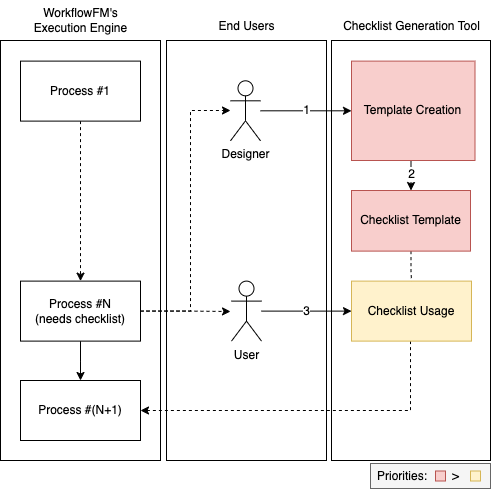
\includegraphics[width=0.65\textwidth]{overleaf/images/overall_system_diagram.png}
    \caption{Overall System Diagram}
    \label{fig:overall_system_diagram}
\end{figure}

\section{Functional Specification}
\label{functional_spec}
According to section \ref{background:chens_design} in Background and discussion with the product owner, we have concluded the functional specification into six functions and three original ideas from ourselves.

\begin{itemize}
    % \item \textbf{Template Creation}
    % \item \textbf{Template Saving}
    % \item \textbf{Checklist Viewing}
    % \item \textbf{Auto Generation*}
    % \item \textbf{Query Suggestion*}
    \item \textbf{Template Creation} is a function for a checklist designer to generate a new checklist template. Given the process details from WorkflowFM, the prototype should return a checklist template, which will be discussed more in section \ref{checklist_strcuture}.
    % \begin{itemize}
    %     \item Checklist's name is, as straight forward as it sounds, the name of this checklist template.
    %     \item Input information is the section that displays information from the values of the process's input data models.
    %     \item Form is the section where displays form components, including textboxes, calendars, dropdown menus, etc. Additionally, all output data models must be linked to every form components through dependencies linking.
    % \end{itemize}
    % This function is for the checklist designer to generate a new suggested template. Given a workflow process from WorkflowFM, the prototype should return a checklist template, which contains three sections: checklist name, input information, and output components.
    % explaining what this spec would do on the user's perspective
    \item \textbf{Input Information Query} is a function that allows a designer to add a new input information to the template. A checklist template allows the designer to add a new input information field to the template. A new input information field needs to be related to the original input information either as a foreign key or a parent key. A checklist template can use input information to query other input information to display in the section.
    % This function allows the designer to add a new input information to the template. A checklist template can use input information to query other input information to display in the section.
    \item \textbf{Form Adjustment} is a function that provides a designer with the flexibility to adjust components inside the form. There are five things a component can be adjusted: name, sequence order, requirability, visibility, and type.
    % Additionally, there are ten possible types of components: {tab}, {header}, {text box}, {paragraph}, {dropdown menus}, {choices}, {check boxes}, {date input}, {time input}, and {constant}.
    % things that can be adjust: type, required, hidden, order, name.
    % This function provides the flexibility to adjust a template to the checklist designer. A checklist template is able to add and adjust a new output component.
    \item \textbf{Dependencies Linking} is a function for a checklist designer to link the input and output dependencies to form components.
    \begin{itemize}
        \item An input dependency is a dependency that, when linked to a form component, causes that form component to connect to the value of the input data model.
        \item An output dependency is a dependency that, when linked to a form component, registers that form component as a component of the output data model.
    \end{itemize}
    % This function is for the checklist designer to link the input and output dependencies together.
    % An output component is able to link with the workflow process.
    \item \textbf{Template Saving} is a function that allows a checklist designer to save the template after finishing adjusting the checklist template.
    % This function is for the checklist designer to save the template after adjusting a checklist template.
    \item \textbf{Checklist Viewing} is a function that allows anyone to access a checklist template that has been created.
    % This function allows anyone to view the template that has been created.
    \item \textbf{Dependencies Validation} is one of the original functions specifically to validate dependencies in form components. It would give an error for every output dependency that is not linked to a form component.
    \item \textbf{Query Recommendation} is one of the original functions that provides an optional recommendation to a checklist designer to get suggested query information rather than manually inserting them one-by-one. The recommendation is based on the existing templates in the system.
    % This function provides the checklist designer an optional recommendation to get suggested query information rather than manually inserting one by one. The recommendation is based on the existing query information in the system.
    \item \textbf{Auto Generation} is one of the original functions that offers an optional automatic form generation on top of the template creation function for a checklist designer. This function automatically builds the whole template as well as links the dependencies based on the data models in from WorkflowFM.
    % This function offers an optional automatical dependency linkage for the checklist designer. The auto-link is based on existing, comparable templates from the system.
\end{itemize}

From the functional specification, we drew an use case diagram to visualise the connections between each function in Figure \ref{fig:use_case_diagram}. It is worth noting that some of the use case may not appear as a functionality in the functional specification, but they are generic enough to be in any system. We also provide sequence diagrams of each scenario in Appendix \ref{appendix:sequence_diagrams}.

\begin{figure}[ht!]
    \centering
    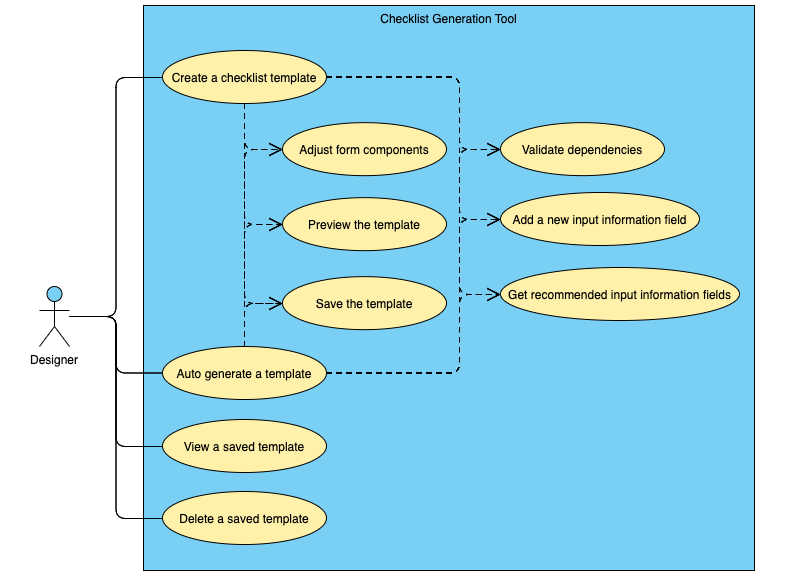
\includegraphics[width=0.8\textwidth]{overleaf/images/use_case_diagram.png}
    \caption{Use Case Diagram}
    \label{fig:use_case_diagram}
\end{figure}



\section{Software's Structure}
\label{design:software_structure}
According to section \ref{functional_spec}, we have grouped and categorised our project, as shown in Figure \ref{fig:software_structure}, into three parts: backend, frontend, and database.

\begin{figure}
    \centering
    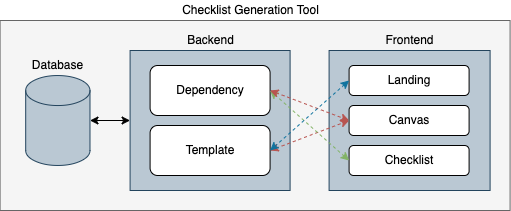
\includegraphics[width=0.7\textwidth]{overleaf/images/software_structure.png}
    \caption{Software's Structure}
    \label{fig:software_structure}
\end{figure}

\begin{itemize}
    \item Backend is the part which prepares and serves information from the database to the frontend. There are three routes as following:
    \begin{itemize}
        \item \textbf{Checklist} is the component that involves checklist-related features. This components only serves \textbf{Checklist Viewing} functionality.
        \item \textbf{Dependency} is the component involving all dependency-related features of the system. This contains \textbf{Input Information Query}, \textbf{Query Recommendation}, and \textbf{Auto Generation} functionalities.
        \item \textbf{Template} is the component involving all template-related features. This contains \textbf{Template Creation} and \textbf{Template Saving}. 
    \end{itemize}
    \item Frontend is an intermediate that allows both designers and workflow users to interact with the backend through web-based application interfaces. There are three main routes as following:
    \begin{itemize}
        \item \textbf{Landing} is the main page of the software. From this component, it could connect to other components in the software. This component connects to Backend's Checklist in order to display checklists' metadata.
        \item \textbf{Canvas} is the component that allows users to interact with the software to create templates from a workflow process. This part connects to both Backend's Dependency and Template in order to retrieve all information to facilitate users to build a template.
        % is the template creation screen. This screen connects to Backend's Denpendency and Template to create and save a template.
        Additionally, this part provides \textbf{Form Adjustment}, \textbf{Dependencies Linking}, and \textbf{Dependencies Validation}.
        \item \textbf{Checklist} is the component that allows people to view a saved checklist template. This component connects to Backend's Checklist to retrieve template's information.
        % is a screen that allows people to view a checklist template through its interface. This screen connects to Backend's Checklist to retrieve a saved checklist template's information.
    \end{itemize}
    \item Database is the storage of the system that stores the data models from WorkflowFM and details of created templates.
\end{itemize}

% Specifically for the screen \#4, we designed the input information and form sections to plan on what features we should be implementing, as seen in Figure \ref{fig:input_info_and_form}.
% This will be discussed more in Implementation.

% \begin{figure}
%     \centering
%     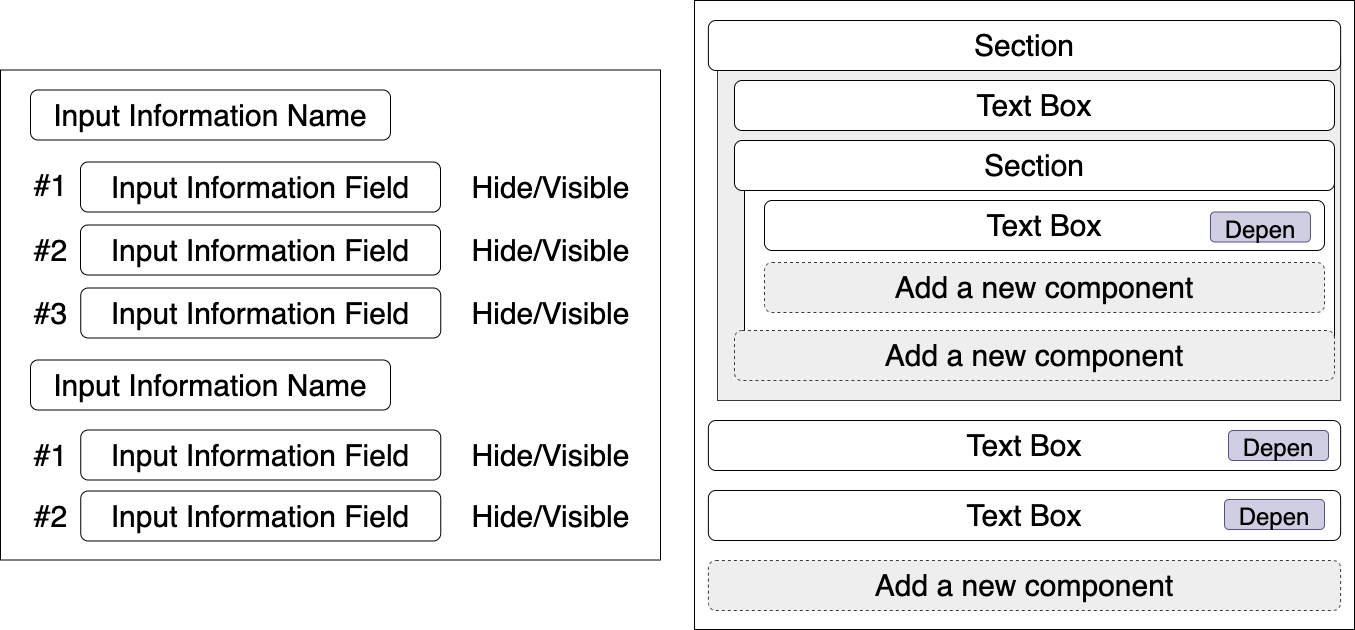
\includegraphics[width=0.9\textwidth]{overleaf/images/input_info_and_form.png}
%     \caption{Input Information's (Left) and Form's (Right) Interface Designs}
%     \label{fig:input_info_and_form}
% \end{figure}
\section{Checklist Template's Structure}
\label{checklist_strcuture}


\begin{figure}[ht!]
    \centering
    \textit{This example will be used to help explain the checklist} template's structure.
    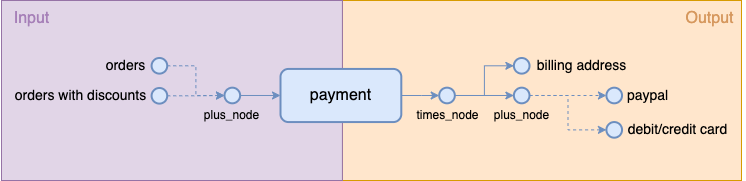
\includegraphics[width=\textwidth]{overleaf/images/template_example.png}
    \caption{Example Process}
    \label{fig:template_example}
\end{figure}

Given an example process in Figure \ref{fig:template_example}, we will assume this payment process needs a checklist for users to fill in billing address and either their debit/credit card information or their PayPal account. This process also has incoming input being either regular orders or orders with discounts.

We will assume that \verb!orders!, being an entity, contains two fields: order id and total price; \verb!orders with discounts! contains three fields: order id, total price, and discount code; \verb!billing address! contains two fields: home address and country; \verb!paypal! contains only paypal account; and \verb!debit/credit card! contains three fields: card number, expire date, and security code.




A checklist template is created by the template creation function. Its purpose is to perform a certain task for workflow users.
A checklist template contains three main parts: the name of the template, the input information, and the form components.

\begin{itemize}
    \item The name of the template is as straightforward as it sounds.
    \item Input information is the inputs' information that comes into the process.
    For example, in Figure \ref{fig:template_example}, the input information of this checklist template are the input part in the diagram: \verb!orders! and \verb!orders with discounts!. It is worth mentioning that being \verb!times! or \verb!plus! does not matter here. Every non-duplicate data model is counted towards input information.
    \item A form component is a representation of a form component, i.e. text boxes, calendars, dropdown menus, etc. For example, in Figure \ref{fig:template_example}, we could be six text boxes to cover everything (i.e. home address, country, paypal account, card number, expire date, and secuirty code).
    % \verb!paypal account!, \verb!debit/credit card number!, and \verb!security code!; and a date input for \verb!expire date!.
\end{itemize}

% As mentioned in Background section \ref{background:input_output}, the template creation only needs the name,  input, and output of the process to generate a checklist template. Thus, we consider all three of them as the template creation's input.
% For example, in Figure \ref{fig:template_example}, the template creation's inputs are shown in Table \ref{tab:process_input}.

% \begin{table}[ht!]
%     \small
%     \begin{tabularx}{\textwidth} { 
%         | p{\dimexpr.3\linewidth-2\tabcolsep-1.3333\arrayrulewidth}
%         | >{\centering\arraybackslash}X | }
%         \hline
%         \textbf{Process Name} & payment\\ 
%         \hline
%         \textbf{Inputs} & plus(orders, orders with discounts) \\
%         \hline
%         \textbf{Outputs} & times(billing address, plus(paypal, debit/credit card)) \\
%         \hline
%     \end{tabularx}
%     \caption{Template Creation's Inputs}
%     \label{tab:process_input}
% \end{table}

% We decided to use a tree data structure for checklist templates in order to. 
% The data models of checklist templates includes ChecklistTemplate, InputInformation, Details, and Component as shown in Figure \ref{fig:data_structure}.
% The checklist template, which is the output of the template creation, is also a repeated children structure (non-binary tree structure), similar to the input because we need to transform filled checklists to the tree structure and send them to the next process after the checklist usage. The input and output diagram is shown in Figure \ref{fig:system_input_output}.

% \begin{figure}[ht!]
%     \centering
%     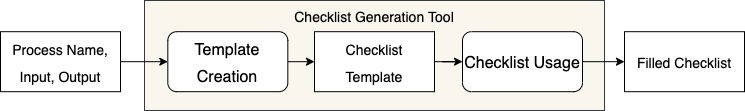
\includegraphics[width=0.8\textwidth]{overleaf/images/system_input_output.png}
%     \caption{System's Input and Output Diagram}
%     \label{fig:system_input_output}
% \end{figure}

% As stated in both \ref{intro:scope_of_work} and \ref{design:overall}, we only focus on the template creation. Thus, we only designed the data structure of the checklist template

We designed four models, as shown in Figure \ref{fig:data_models}, to represent the three main parts of a checklist template based on the functionalities in section \ref{functional_spec} and used these models across the system. Furthermore, the database was also designed based on these models, which the actual database design can be seen in Appendix \ref{fig:checklist_db_design}.
% Additionally, the relation between models and functions can be seen in Table \ref{tab:model_to_function}.
% Four models were designed to represent the three main parts of a checklist template as shown in Figure \ref{fig:data_models}.
\begin{itemize}
    \item ChecklistTemplate is a model representing the overall structure of a checklist template. It contains two other models inside: InputInformation and Component.
    \item InputInformation is a model representing the input information metadata of a checklist template, e.g. \verb!orders! and \verb!orders with discounts!. It contains Details model inside to the fields in the input information.
    \item Details represents a input information field under InputInformation. For example, order id and total price in \verb!orders!; and home address and country in \verb!billing address!.
    \item Component is model representing a form component in a template. For example, as shown in Figure \ref{fig:component_example}, we could have two root components which are sections. The first section is to represent the billing address, and the other one is to represent the payment methods (PayPal and card). Under the billing address section, it contains two text boxes of home address and country. Under the payment methods, it contains two more sections of PayPal and Card, which they contain fields inside.
    % is a tree-structured model representing a form component in a template. Additionally, it can recursively contain itself as children.
\end{itemize}


\begin{figure}[ht!]
    \centering
    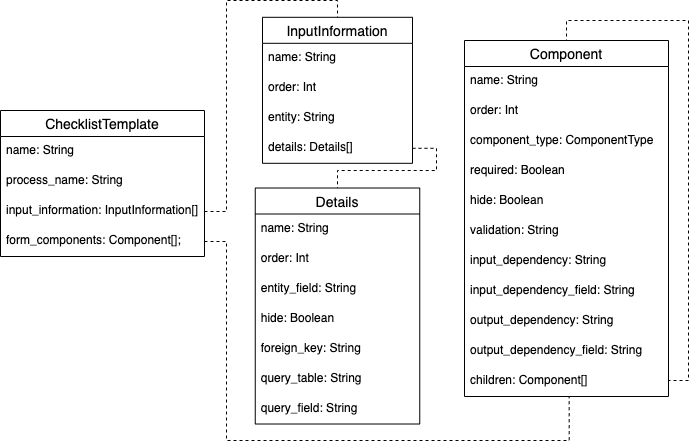
\includegraphics[width=0.9\textwidth]{overleaf/images/data_models.png}
    \caption{Checklist Template's Data Models}
    \label{fig:data_models}
\end{figure}

It is worth mentioning that the component model is a tree, similar to WorkflowFM's input and output. The rationale is for convenience for the auto generation function, which will be discussed in more detail in the Implementation chapter.

\begin{figure}[ht!]
    \centering
    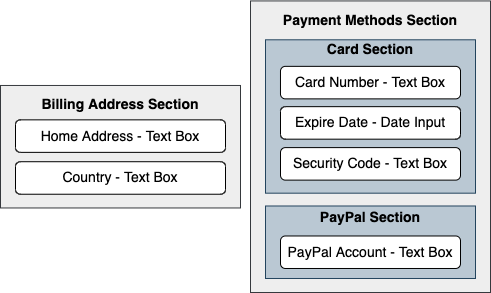
\includegraphics[width=0.6\textwidth]{overleaf/images/component_example.png}
    \caption{Example of Components}
    \label{fig:component_example}
\end{figure}

\section{Interface Design}
\label{interface_design}
We designed the interfaces of this project based on Chen's design \cite{checklistdesign} and popular form generators, such as Google Forms \cite{googleforms} and Microsoft Forms \cite{msforms}. We used Chen's design as the base design for the functionalities in the website and modernised the design based on the designs of popular platforms. The sketch of how each interface navigates is shown in Figure \ref{fig:overall_interface_design}.

\begin{figure}[ht!]
    \centering
    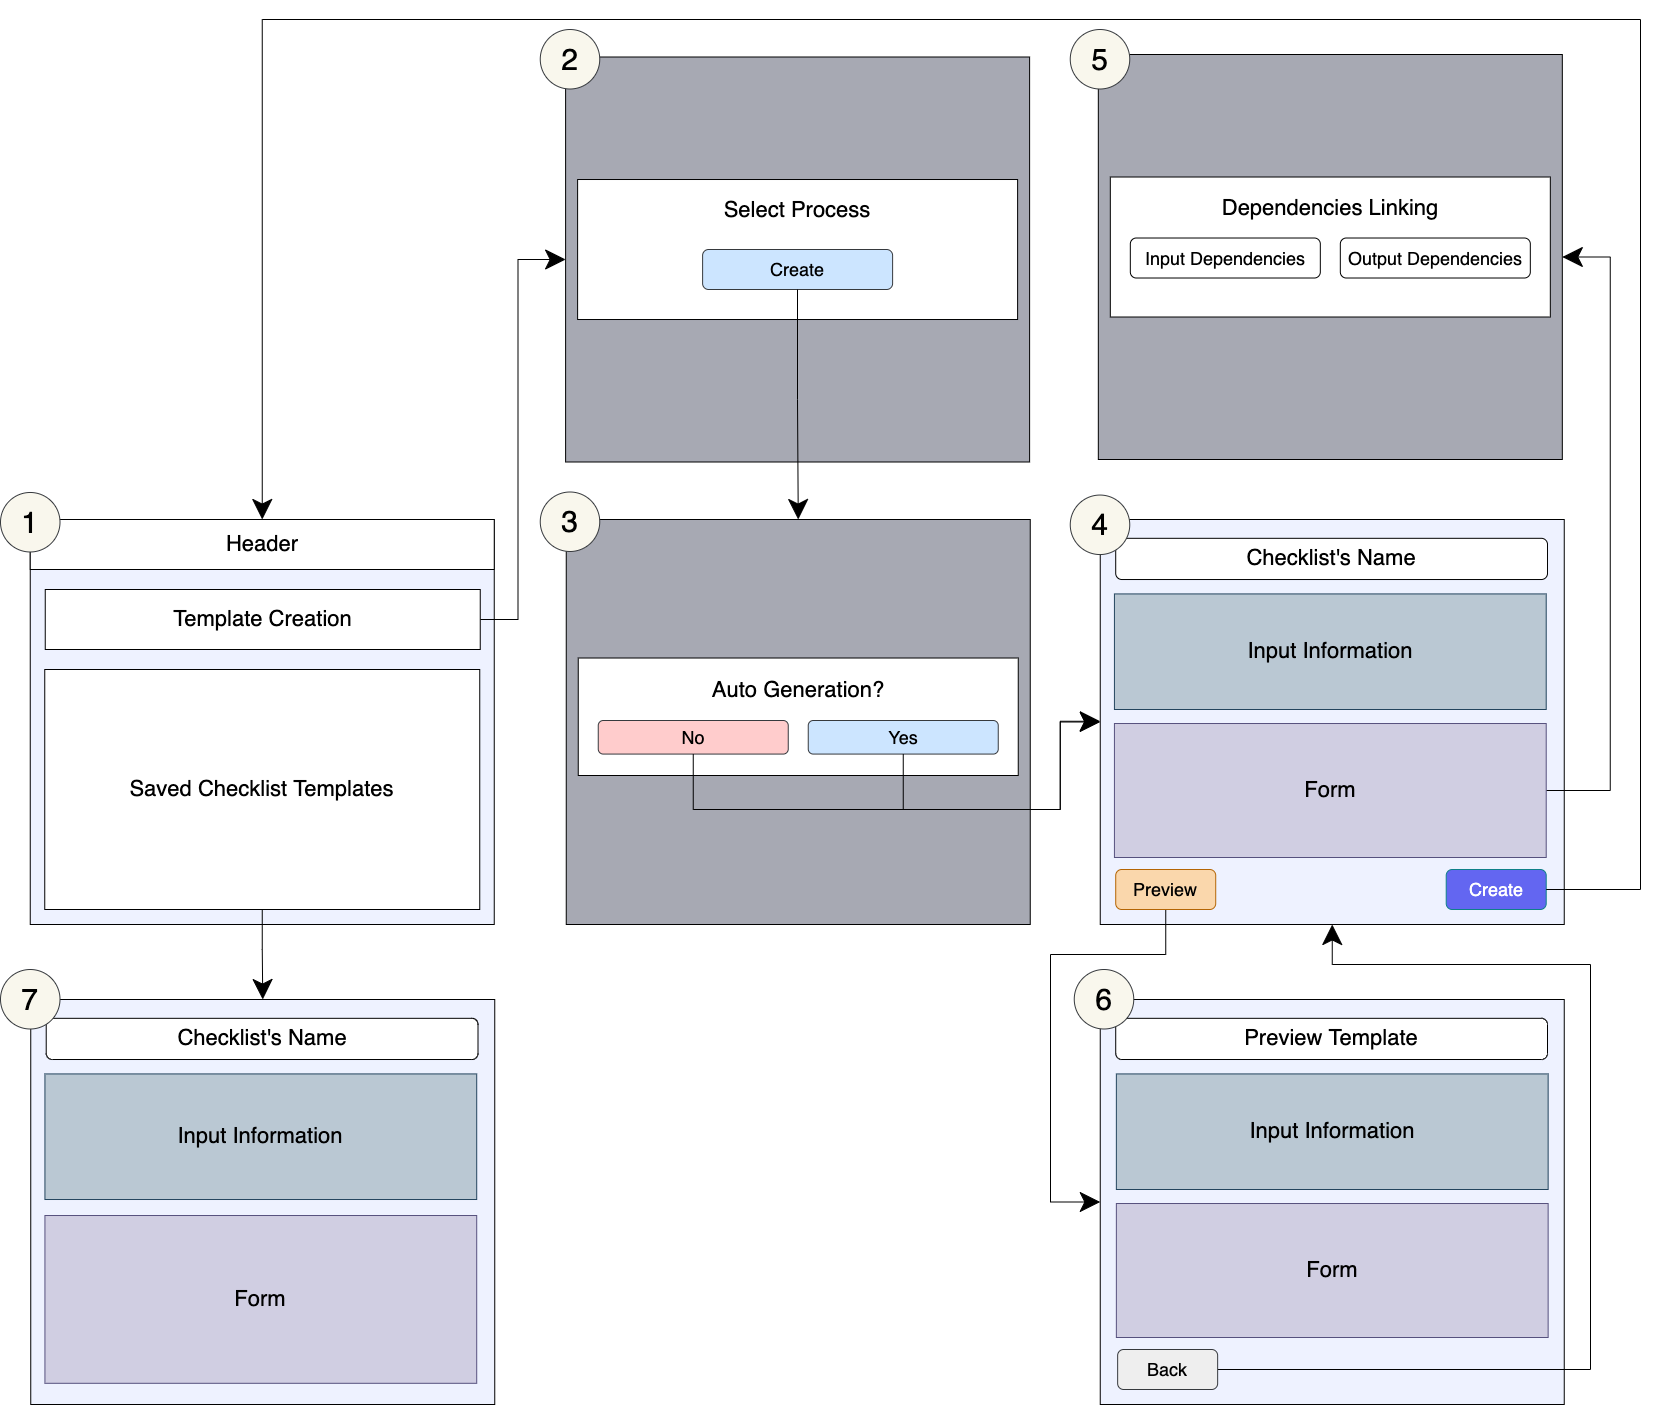
\includegraphics[width=\textwidth]{overleaf/images/overall_interface_design.png}
    \caption{Overall Interface Design}
    \label{fig:overall_interface_design}
\end{figure}

From the sketch, it can be seen that there are only three different screens (screens \#1, \#4, and \#8), one duplicated screens (screen \#6), and four popup screens (screens \#2, \#3, \#5, and \#7). Starting from screen \#1, this is the landing page (the main screen) that contains two sections: template creation and saved checklist templates. The template creation section will navigate users to screen \#2 to create a new template. Meanwhile, The saved templates section displays a list of saved templates in the system and will let users navigate to screen \#8 to view a saved template.

On screens \#2 and \#3, they are both popups that allow users to i) select a workflow process that users want to create a template for; and ii) select whether or not users want to use the template auto-generation to generate the template.

Screen \#4 is the canvas screen. This screen allows users to create or adjust the checklist template of the process that they select in screen \#2. There are three sections in this screen, including the checklist's name section, the input information section, and the form adjustment section. The details of each section will be explained in the Implementation chapter.
Screen \#4 can navigate to screen \#5 through the form section. Screen \#5 is a popup screen to manage dependencies for the dependencies linking function.

% Screen \#4 is the canvas screen. This screen allows users to create or adjust the checklist template of the process that they select in screen \#2. There are three sections in this screen, including the checklist's name section, the input information section, and the form section. The input information section consists of the name and fields of the input information, as shown in Figure \ref{fig:input_info_and_form} (Left). The form section consists of a group of components, as seen in Figure \ref{fig:input_info_and_form} (Right). A component can be one of the ten types: header, tab, textbox, paragraph, dropdown, choices, checkboxes, date, time, and constant. Additionally, header and tab components can contain a group of components.


Screen \#6 is a preview screen of the template that a user creates in screen \#4. It follows the same structure as screen \#4, but users are not allowed to adjust anything on this screen. Additionally, this screen has the same design as screen \#8. Users can navigate to this screen through the preview button and navigate back via the back button.

Users can save the template using the create button on screen \#4. This will navigate to a popup on screen \#7, which will eventually navigate back to screen \#1. After arriving on screen \#1, users should see the template they create displaying on the saved checklist templates section.

% From the sketch, it is obvious that there are only three different screens, one duplicated screen, and four popup screens. Starting from screen \#1, this is the landing page (the main screen) that contains two sections: template creation and saved checklist templates. The template creation section will navigate users to screen \#2 to create a new template. The saved templates section displays a list of saved templates in the system, and will let users navigate to screen \#8 to view a saved template.
% This screen contains three parts as follow to the checklist template's structure, which will be clarified more in section \ref{checklist_strcuture}.


% \begin{figure}[ht!]
%     \centering
%     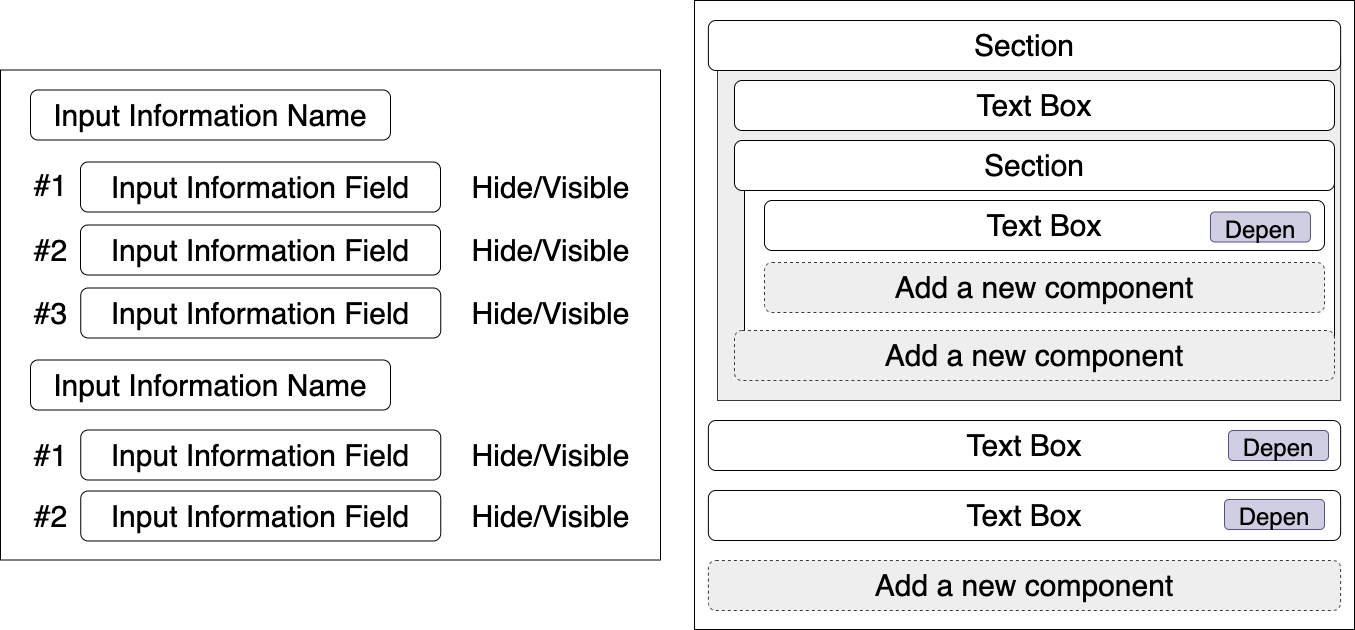
\includegraphics[width=0.65\textwidth]{overleaf/images/input_info_and_form.png}
%     \caption{Input Information's (Left) and Form's (Right) Interface Designs}
%     \label{fig:input_info_and_form}
% \end{figure}

% \section{Database Design}
% - main checklist design

% - templates, components

% - input\_information\_parent, input\_information\_child, input\_information\_child\_query





% \section{Use Case Diagram}





\chapter{Implementation}


\section{Technologies}

\subsection{Frontend}
% Three languages can be used to implement the frontend while using one of the main popular frameworks. This consists of i) JavaScript \cite{javascript}, ii) TypeScript \cite{typescript} and iii) Scala.js \cite{scalajs}. We decided to avoid JavaScript due to the lack of type support. Between TypeScript and Scala.js, we ended up choosing TypeScript over Scala.js. That is because we are more familiar with TypeScript than Scala.js. Moreover, the advantages of Scala.js, according to their website \cite{scalajs}, do not provide much more facilities than what TypeScript has already done. Therefore, TypeScript is selected as our main language to implement the frontend.

% With regard to the frontend framework, there were three frameworks that we considered. Unlike the main language, we are familiar with all three frameworks. Angular \cite{angular} is a large framework with extensive pre-built tools and libraries. However, we decided not to use Angular, because this would have made our frontend unnecessarily large.

% Vue.js \cite{vue} is another popular framework with a large community similar to React \cite{react}. However, Vue.js is not as widely used as React, according to the number of available repository results on GitHub \cite{reactsearch, vuesearch}. That means React has a bigger community that we can rely on. Hence, we decided to use React as our frontend framework.

% According to the concept design \cite{checklistdesign}, the frontend consists of four main screens as follows: \vspace{-8pt}
% Three frontend programming languages to be considered includes: i) JavaScript \cite{javascript}, ii) TypeScript \cite{typescript}, and iii) Scala.js \cite{scalajs}. Although JavaScript and TypeScript are identical in virtually every way, JavaScript does not support static typing. Therefore, we decided to remove JavaScript from the list due to the absence of type support. Scala.js was added to the list because WorkflowFM was using Scala as the backend programming language. However, due to the lack of expertise with Scala.js, we decided to stick with what we were familiar with, which was TypeScript.

TypeScript \cite{typescript} was selected as the programming language for the frontend. That was because we were familiar with TypeScript and its frameworks. 
Although JavaScript \cite{javascript} and TypeScript are identical in virtually every way, JavaScript does not support static typing. Static typing is important to detect potential bugs or errors in the codebase. That was another reason that we chose TypeScript over other languages.

Next.js \cite{nextjs} was chosen as the frontend framework. Next.js is a framework on top of React \cite{react}, a widely used frontend framework, and improves upon it. For the fact that React has the biggest community among frontend frameworks, being React-based would help us if we get stuck somewhere during the implementation.

% Even though the programming language had been decided, we had to select the framework for the prototype. There were three frameworks to be considered: i) Angular \cite{angular}, ii) Nuxt.js (Vue) \cite{nuxtjs, vue}, and iii) Next.js (React) \cite{nextjs, react}. In the end, we decided to use Next.js, which is a framework on top of React, because React has the biggest community among the three, which would be convenient if we get stuck somewhere with the framework.

As Next.js was chosen, Redux \cite{redux} was automatically determined as the state management tool. Redux is centralised storage for all components in an application specifically made for React library.

Finally, we had to decide on the CSS framework among various options. Since we prioritised the flexibility in CSS customisation, we chose TailwindCSS \cite{tailwindcss} as the CSS framework for this project. In contrast to other frameworks, TailwindCSS only offers pre-built classes, not components. This gave us the customisation we wanted.

\subsection{Backend}
The backend programming language was decided to be Scala \cite{scala} because WorkflowFM's execution engine was also using Scala. Using the same language would make the integration between our system and WorkflowFM easier.

As for the framework, we originally planned to use http4s \cite{http4s}. However, due to some technical issues, we could not deploy a http4s project to a cloud service for a quick test in the beginning. Thus, we migrated the framework to Akka-http \cite{akka}. After a quick deployment, Akka-http worked perfectly fine. That is why we chose Akka-http as our backend framework.

% The language that we select to implement the backend of the project is Scala. The reason that we choose Scala over other languages is that WorkflowFM's execution engine is currently using Scala. Hence, using the same language will make it easier to integrate with the execution engine.

% Http4s \cite{http4s} is selected as the framework for the backend. This is because we decide to use RESTful \cite{richardson2008restful} as the protocol to communicate between the server and the client. In fact, there were multiple options that we were considering. However, each of them does not suit well with what we want to do.\vspace{-8pt}

% \begin{itemize}
%     \item Vertx \cite{vertx} is a large framework and has multiple variations in JVM languages. And because of that, Vertx is unnecessary large and not specifically built for functional programming compared to other frameworks.
%     \item Cask \cite{cask} is a microframework. However, Cask is still very young and is not widely used compared to other frameworks. Considering that we are new to Scala, we decided to use other frameworks to avoid unexpected circumstances.
%     \item Akka \cite{akka} is very similar to http4s in terms of community and library size. However, http4s has slightly bigger community than Akka's. Therefore, we decided to use http4s instead.
%     % due to the lack of details in Akka's documentation, we decided to use http4s instead.
% \end{itemize}

% \vspace{-8pt}Therefore, http4s is chosen because it is the most suitable framework compared to other alternatives.


\subsection{Database}
% PostgreSQL was our choice as the database of the system because i) it is a relational database
Originally, we planned to use SQLite \cite{sqlite} as the database since Chen's healthcare database was provided in SQLite. However, the majority of service providers did not offer strong support for SQLite. Because we intended to host the entire project online, we chose to switch the database to PostgreSQL \cite{postgresql}. PostgreSQL is a relational database, much like SQLite, but it is widely used by many developers and has tons of support from cloud providers. This will be helpful if we ever migrate our database later on.
We decided to use PostgreSQL as a service called ElephantSQL \cite{elephantsql} because our prototype was still in the minimum viable product (MVP) stage and could use the service in its free tier.


\subsection{Continuous Integration and Continuous Deployment (CI/CD)}

Since we hosted our codebase on GitHub \cite{github}, it was simple to use GitHub Actions \cite{githubactions} as the continuous integration of our project. As for the continuous deployment, we hosted the frontend on Vercel \cite{vercel} and the backend on Heroku \cite{heroku}, which both provided the continuous deployment service integrated into GitHub.

% \begin{itemize}
%     \item Miscellaneous
%     \begin{itemize}
%         \item GitHub
%         \item GitHub Actions
%         \item PostgreSQL
%         \item ElephantSQL
%         \item Vercel
%         \item Heroku
%     \end{itemize}
% \end{itemize}

% - choices: React, Vue, Angular, Scala.js

% - chose: React, Next.js, TailwindCSS, Redux

% - choices: Node.js, Scala, Java

% - choices for Scala: akka-http, http4s, play

% chose: Scala, Akka-http

% - GitHub, GitHub Actions, PostgreSQL, ElephantSQL, Vercel, Heroku


\section{Frontend}
The implementation of the frontend was based on Design sections \ref{design:software_structure} and \ref{interface_design}. The routing was divided based on section \ref{design:software_structure}, while the navigation and interfaces were based on section \ref{interface_design}.
This prototype is hosted online and can be accessed through \href{https://resource-based-checklist-generation.vercel.app/}{HERE}.

\subsection{Landing}
\label{im:landing}

As mentioned in Design sections \ref{design:software_structure}, this is the main screen of this web application. The navigation from the main screen to the canvas screen follows the navigation in Design section \ref{interface_design}.
It connects the canvas screen (\ref{im:canvas_screen}) through the \verb!Create a New Template! button in the middle-top of the screen, as shown in Figure \ref{fig:main_screen}, following with the process selection popup (Figure \ref{fig:process_input}) and the auto-generation popup (Figure \ref{fig:autogen}).
% The bottom section is a list of saved checklist templates. Each template
Furthermore, this screen allows users to access the view checklist screen (\ref{im:view_checklist}) through selecting a template in the list of saved checklist templates in the bottom section.
% The main screen requires the connection to Backend's Checklist, according to Design section \ref{design:software_structure}, because it needs to display a list of saved checklist templates as shown in the bottom section of Figure \ref{fig:main_screen}.

% call template creation on the popup, 
% call auto generation on the popup
\begin{figure}[ht!]
    \centering
    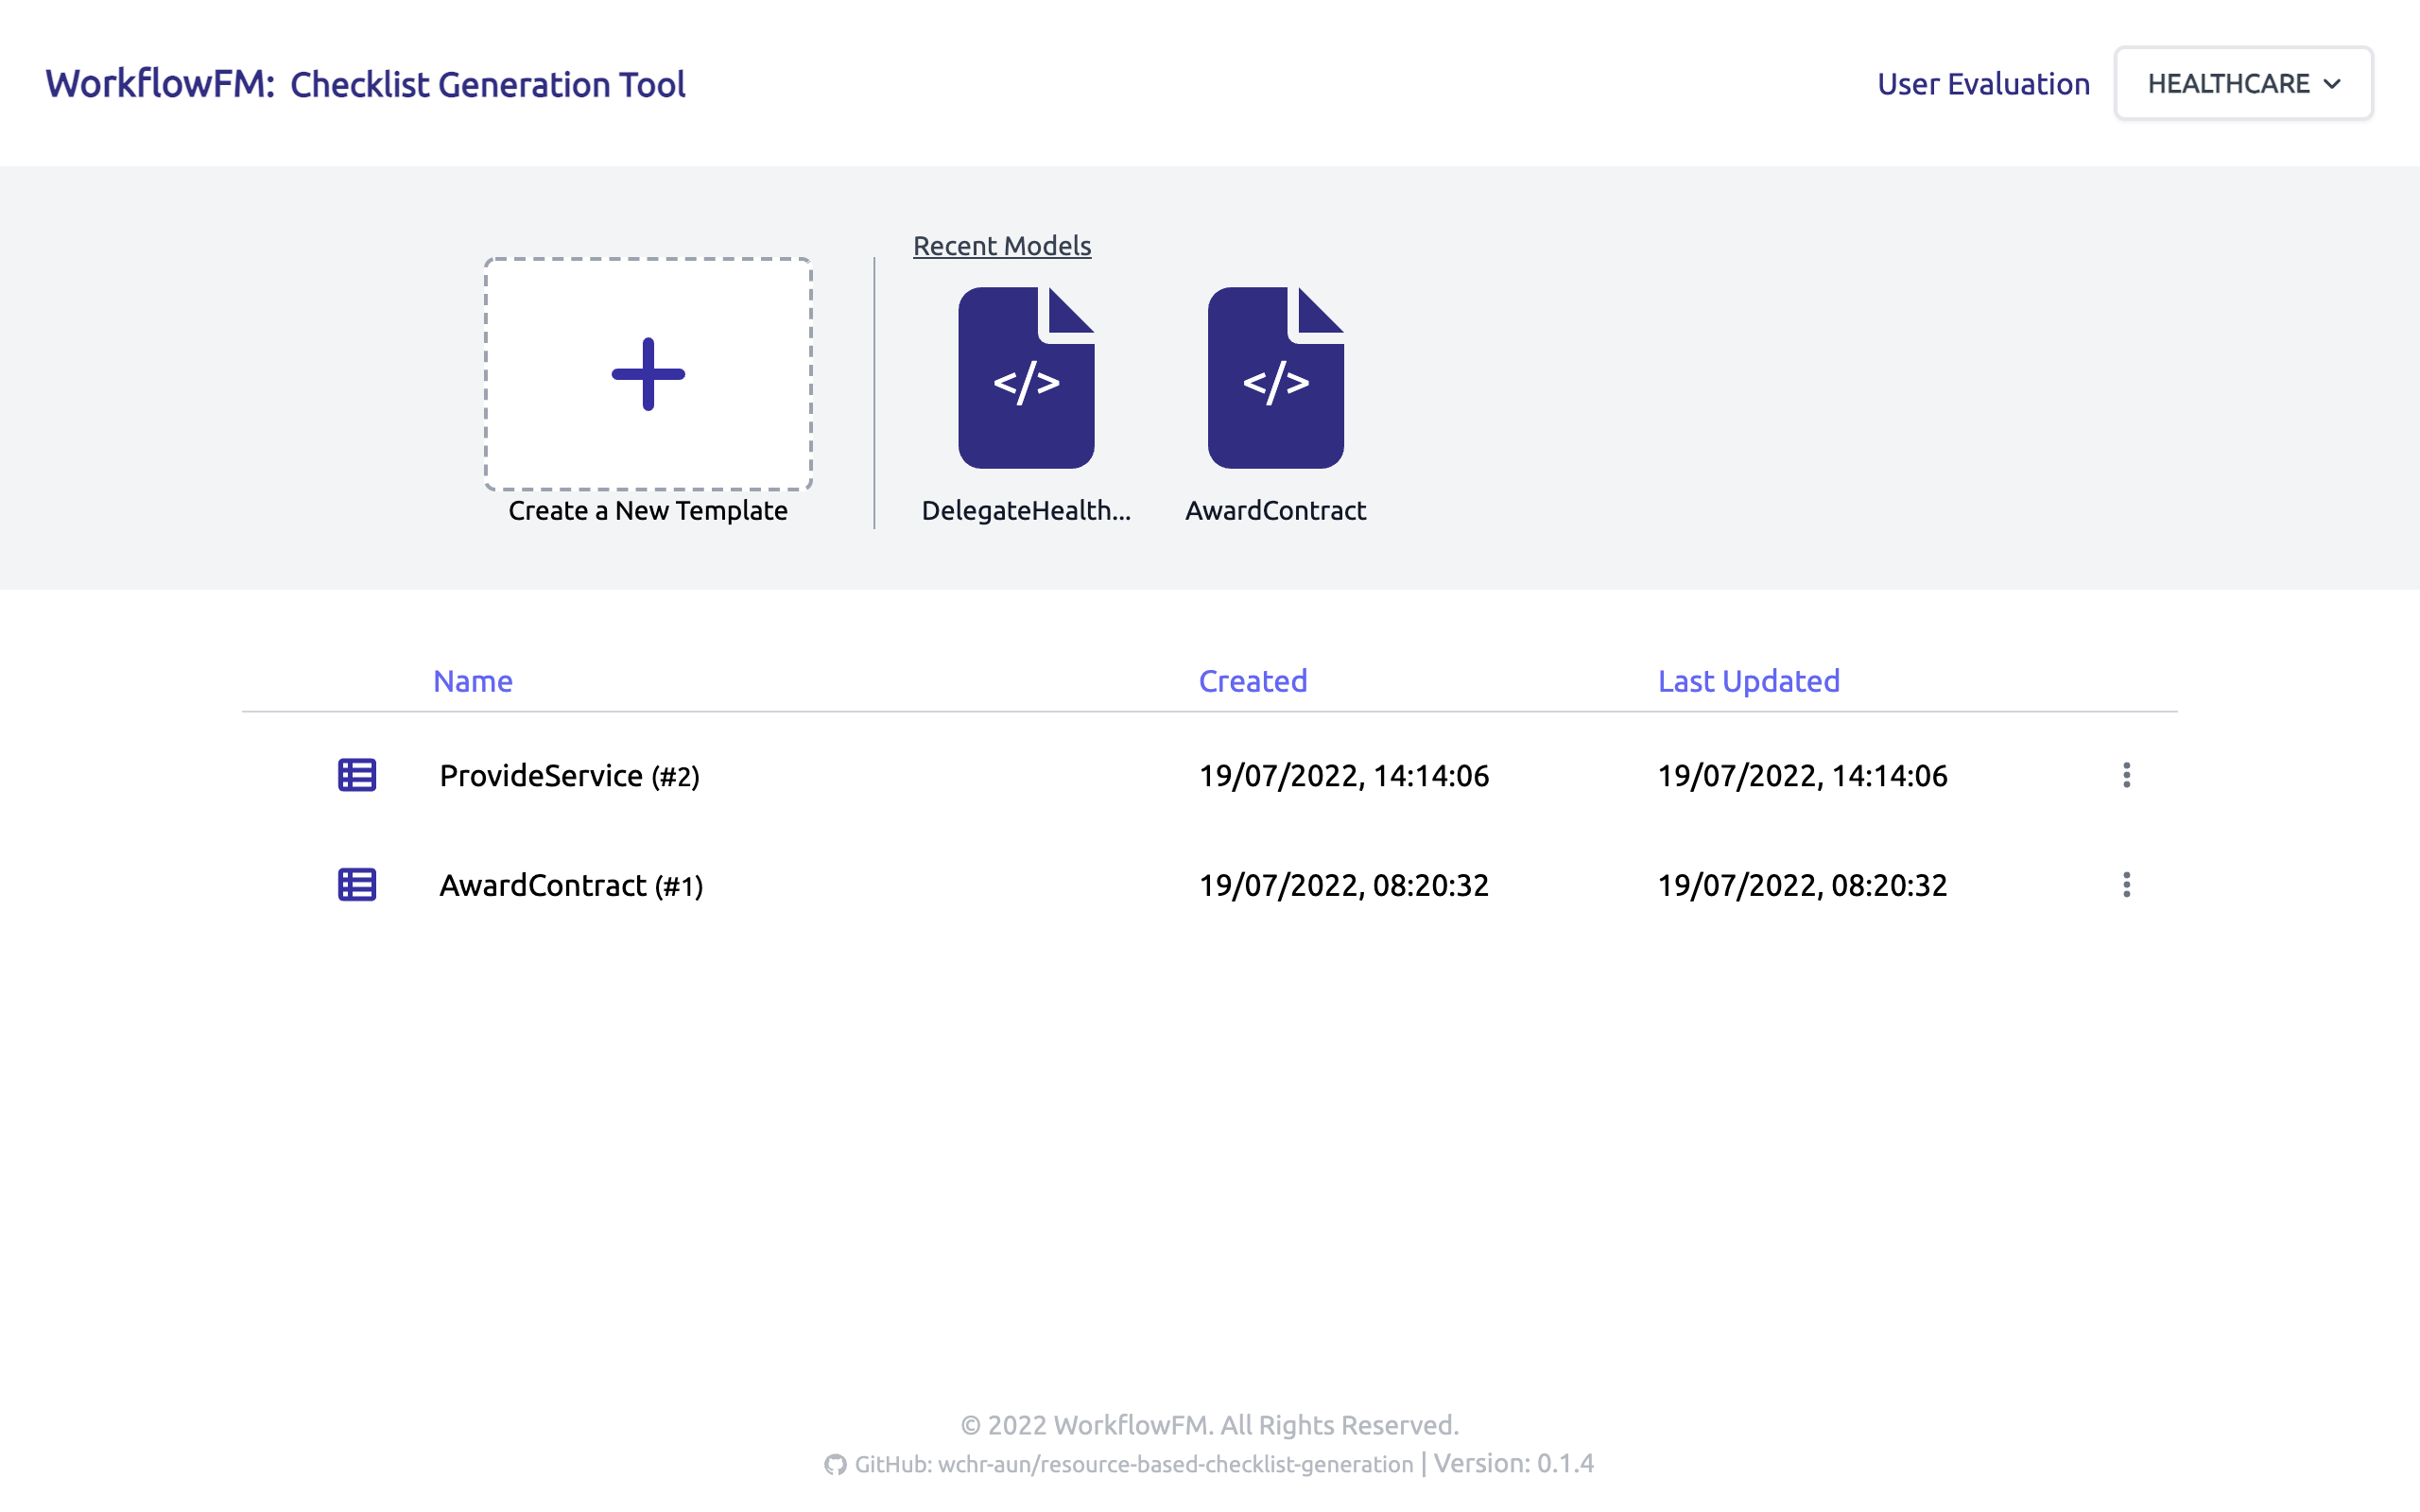
\includegraphics[width=0.6\textwidth]{overleaf/images/screens/main_screen.png}
    \caption{Main Screen}
    \label{fig:main_screen}
\end{figure}


\begin{figure}[ht!]
\centering
\begin{minipage}{.5\textwidth}
  \centering
  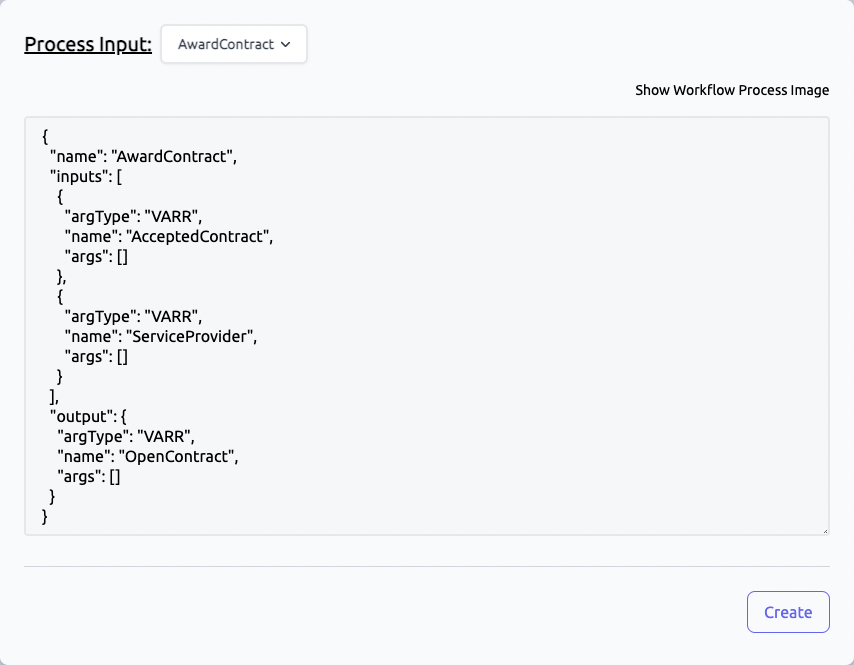
\includegraphics[width=0.9\linewidth]{overleaf/images/screens/process_input.png}
  \caption{Select Process Popup}
  \label{fig:process_input}
\end{minipage}%
\begin{minipage}{.5\textwidth}
  \centering
  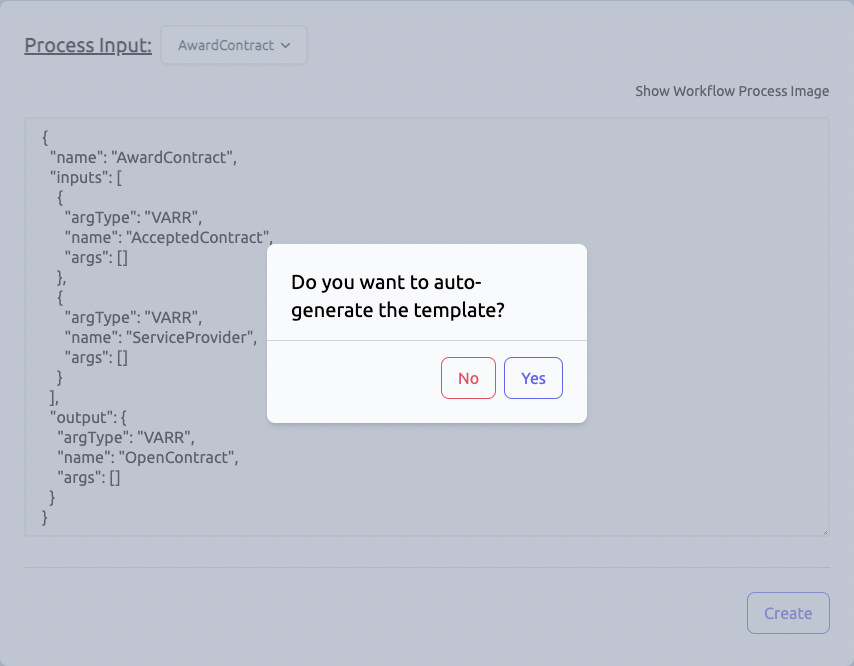
\includegraphics[width=0.9\linewidth]{overleaf/images/screens/autogen.png}
  \caption{Auto-Generation Popup}
  \label{fig:autogen}
\end{minipage}
\end{figure}




\subsection{Canvas}
\label{im:canvas}

In this section, we implemented three screens: Canvas Screen, Dependencies Management Popup, and Preview Screen. Similarly to section \ref{im:landing}, we followed the navigation between these screens from section \ref{interface_design} in Design.


% input information query here,
% query recommendation here,
% template saving here

\subsubsection{Canvas Screen}
\label{im:canvas_screen}

% This screen covers five functionalities, according to the software's structure section \ref{design:software_structure}: Template Creation, Input Information Query, Form Adjustment, Template Saving, and Query Recommendation.
% mention what this screen covers functionalities

As seen in Figure \ref{fig:canvas_screen}, the canvas screen contains three sections: checklist’s name, input information, and form adjustment. These sections are implemented following the checklist template's structure in section \ref{checklist_strcuture}. The display name of each section can be edited. Other than the display names, the input information and the form adjustment sections can adjust the sequence order of what appears before or after as well as the visibility of each field, as shown in Figures \ref{fig:input_information_section} and \ref{fig:form_section}.

% \begin{figure}[ht!]
%     \centering
%     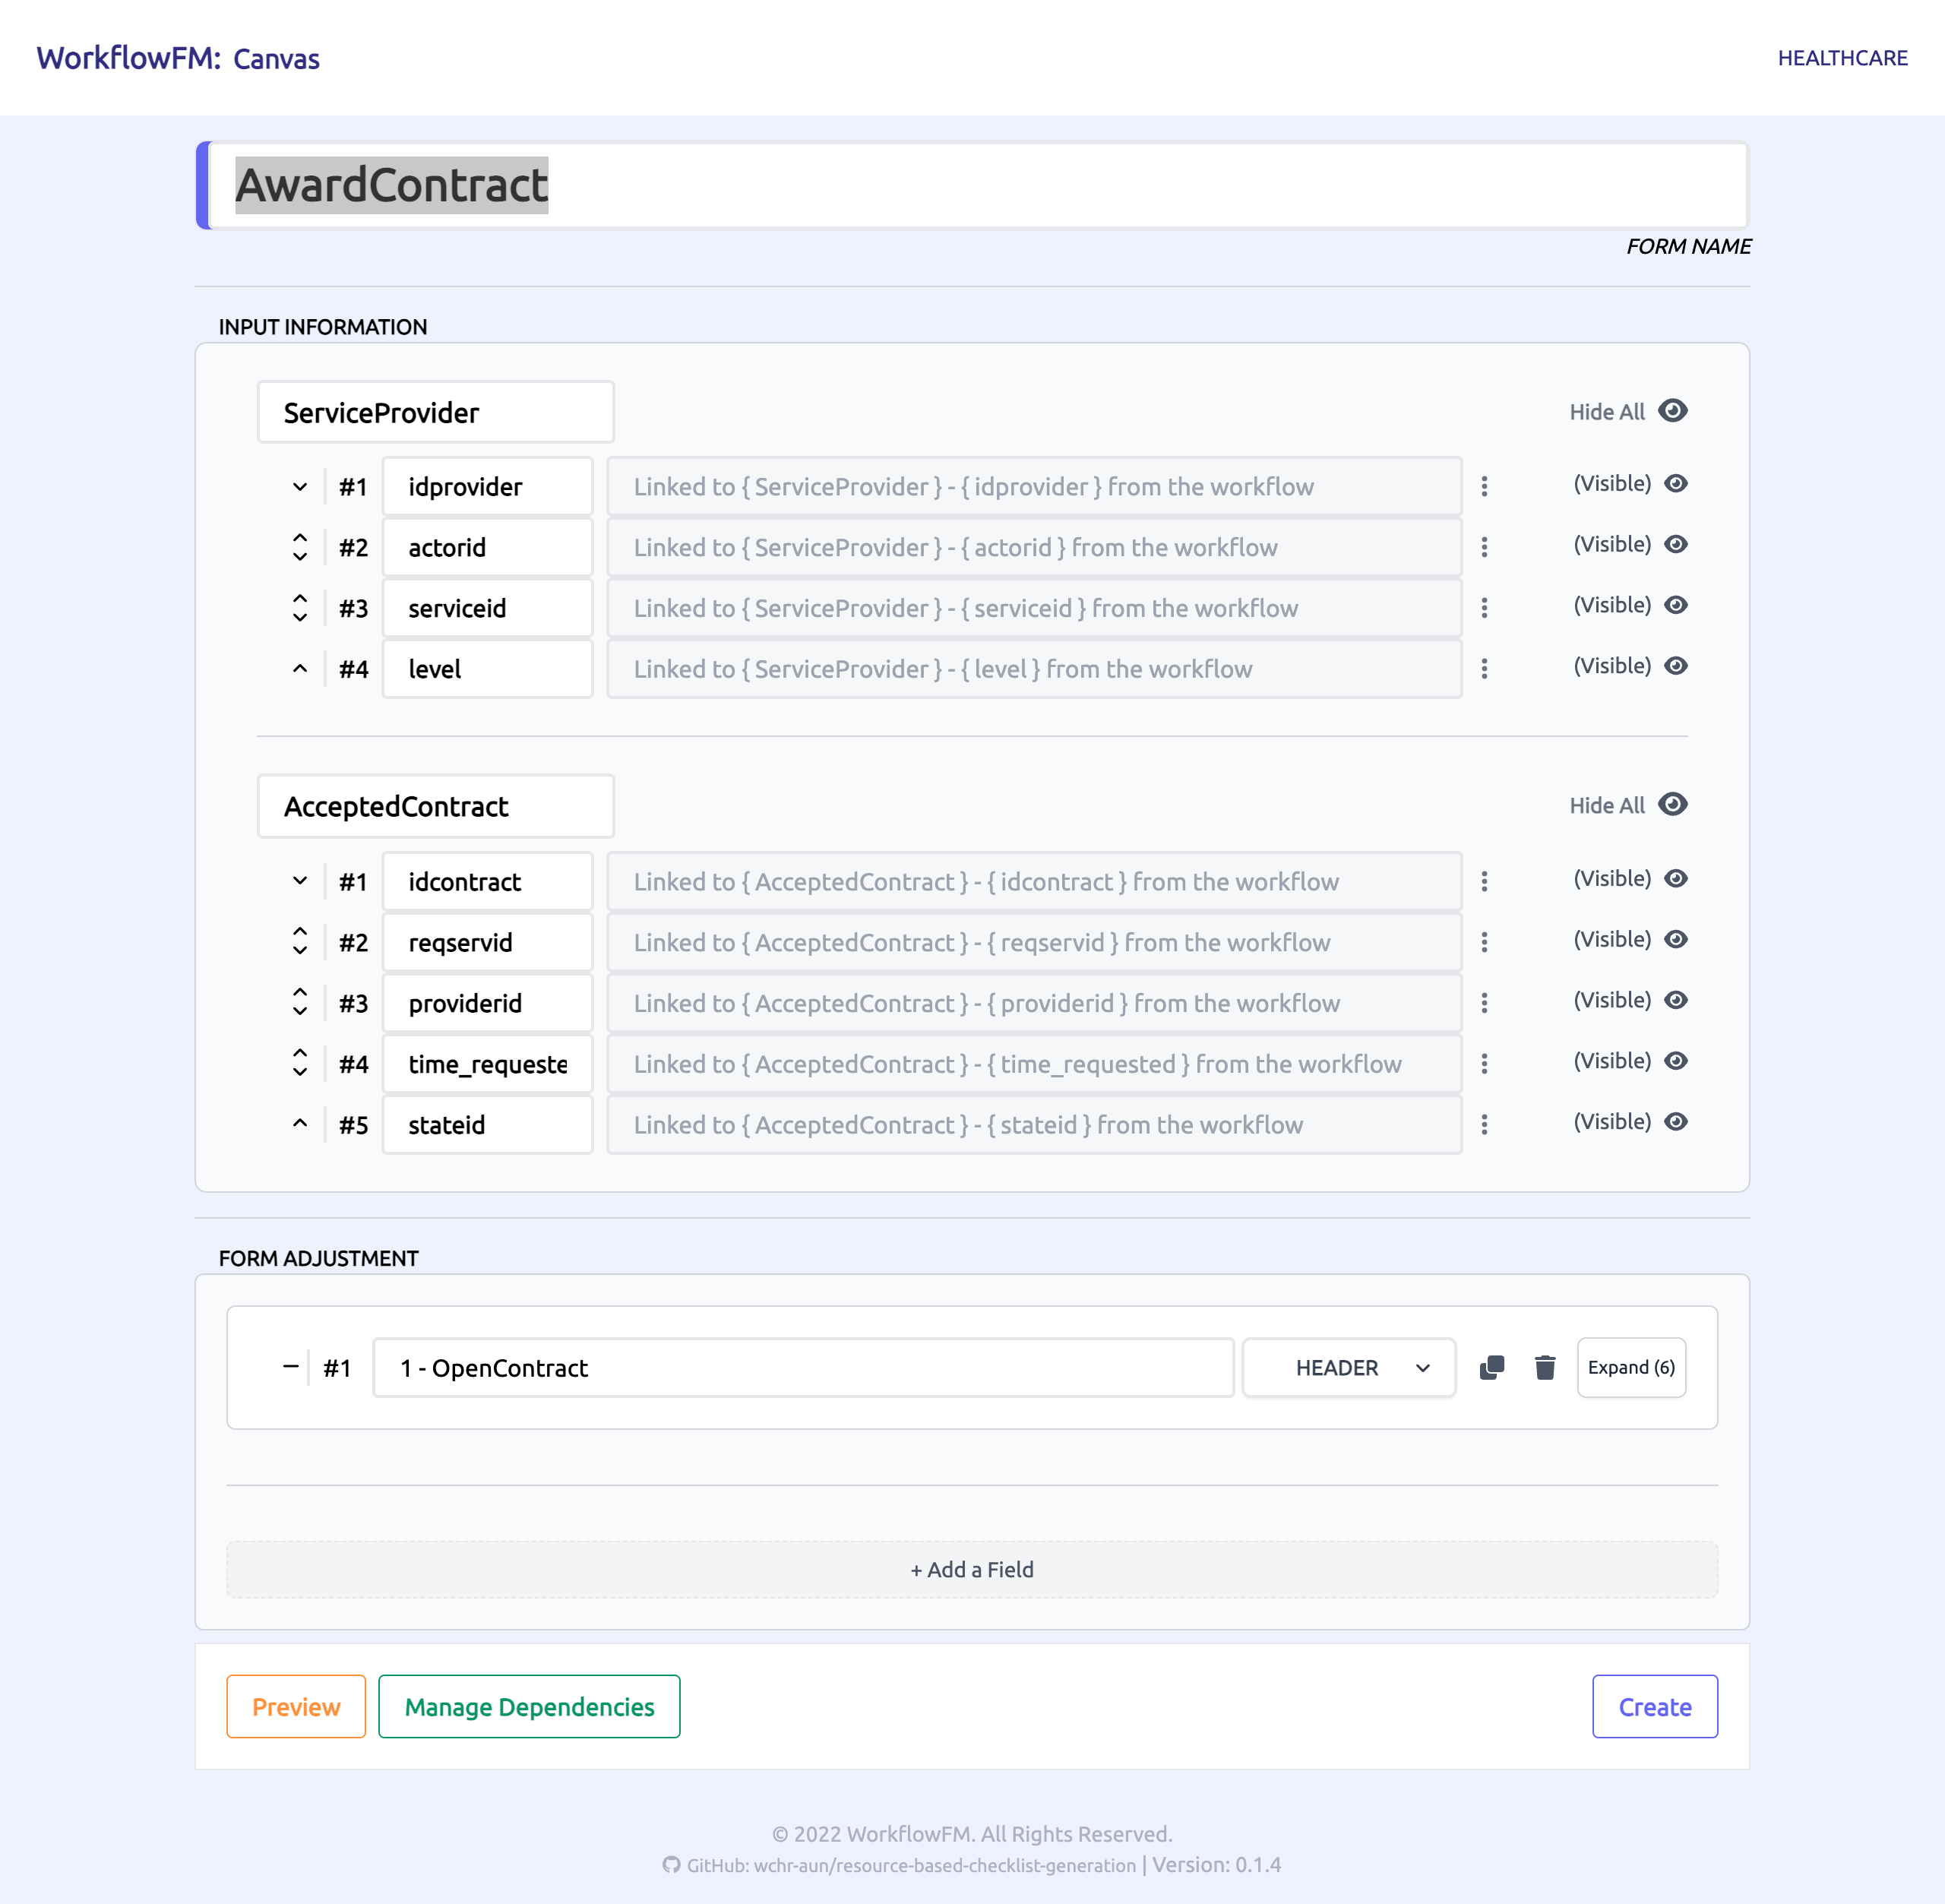
\includegraphics[width=0.6\textwidth]{overleaf/images/screens/canvas_screen.png}
%     \caption{Canvas Screen}
%     \label{fig:canvas_screen}
% \end{figure}

% form adjustment here
Designers can change the component type and the requirability of a component in the form adjustment section. There are ten component types: header, tab, textbox, paragraph, dropdown, choices, checkboxes, date, time, and constant. In addition, a new component can be added via the button at the bottom of each component. This all together is the \textbf{Form Adjustment} functionality.

\begin{figure}[ht!]
\centering
\begin{minipage}{.5\textwidth}
  \centering
  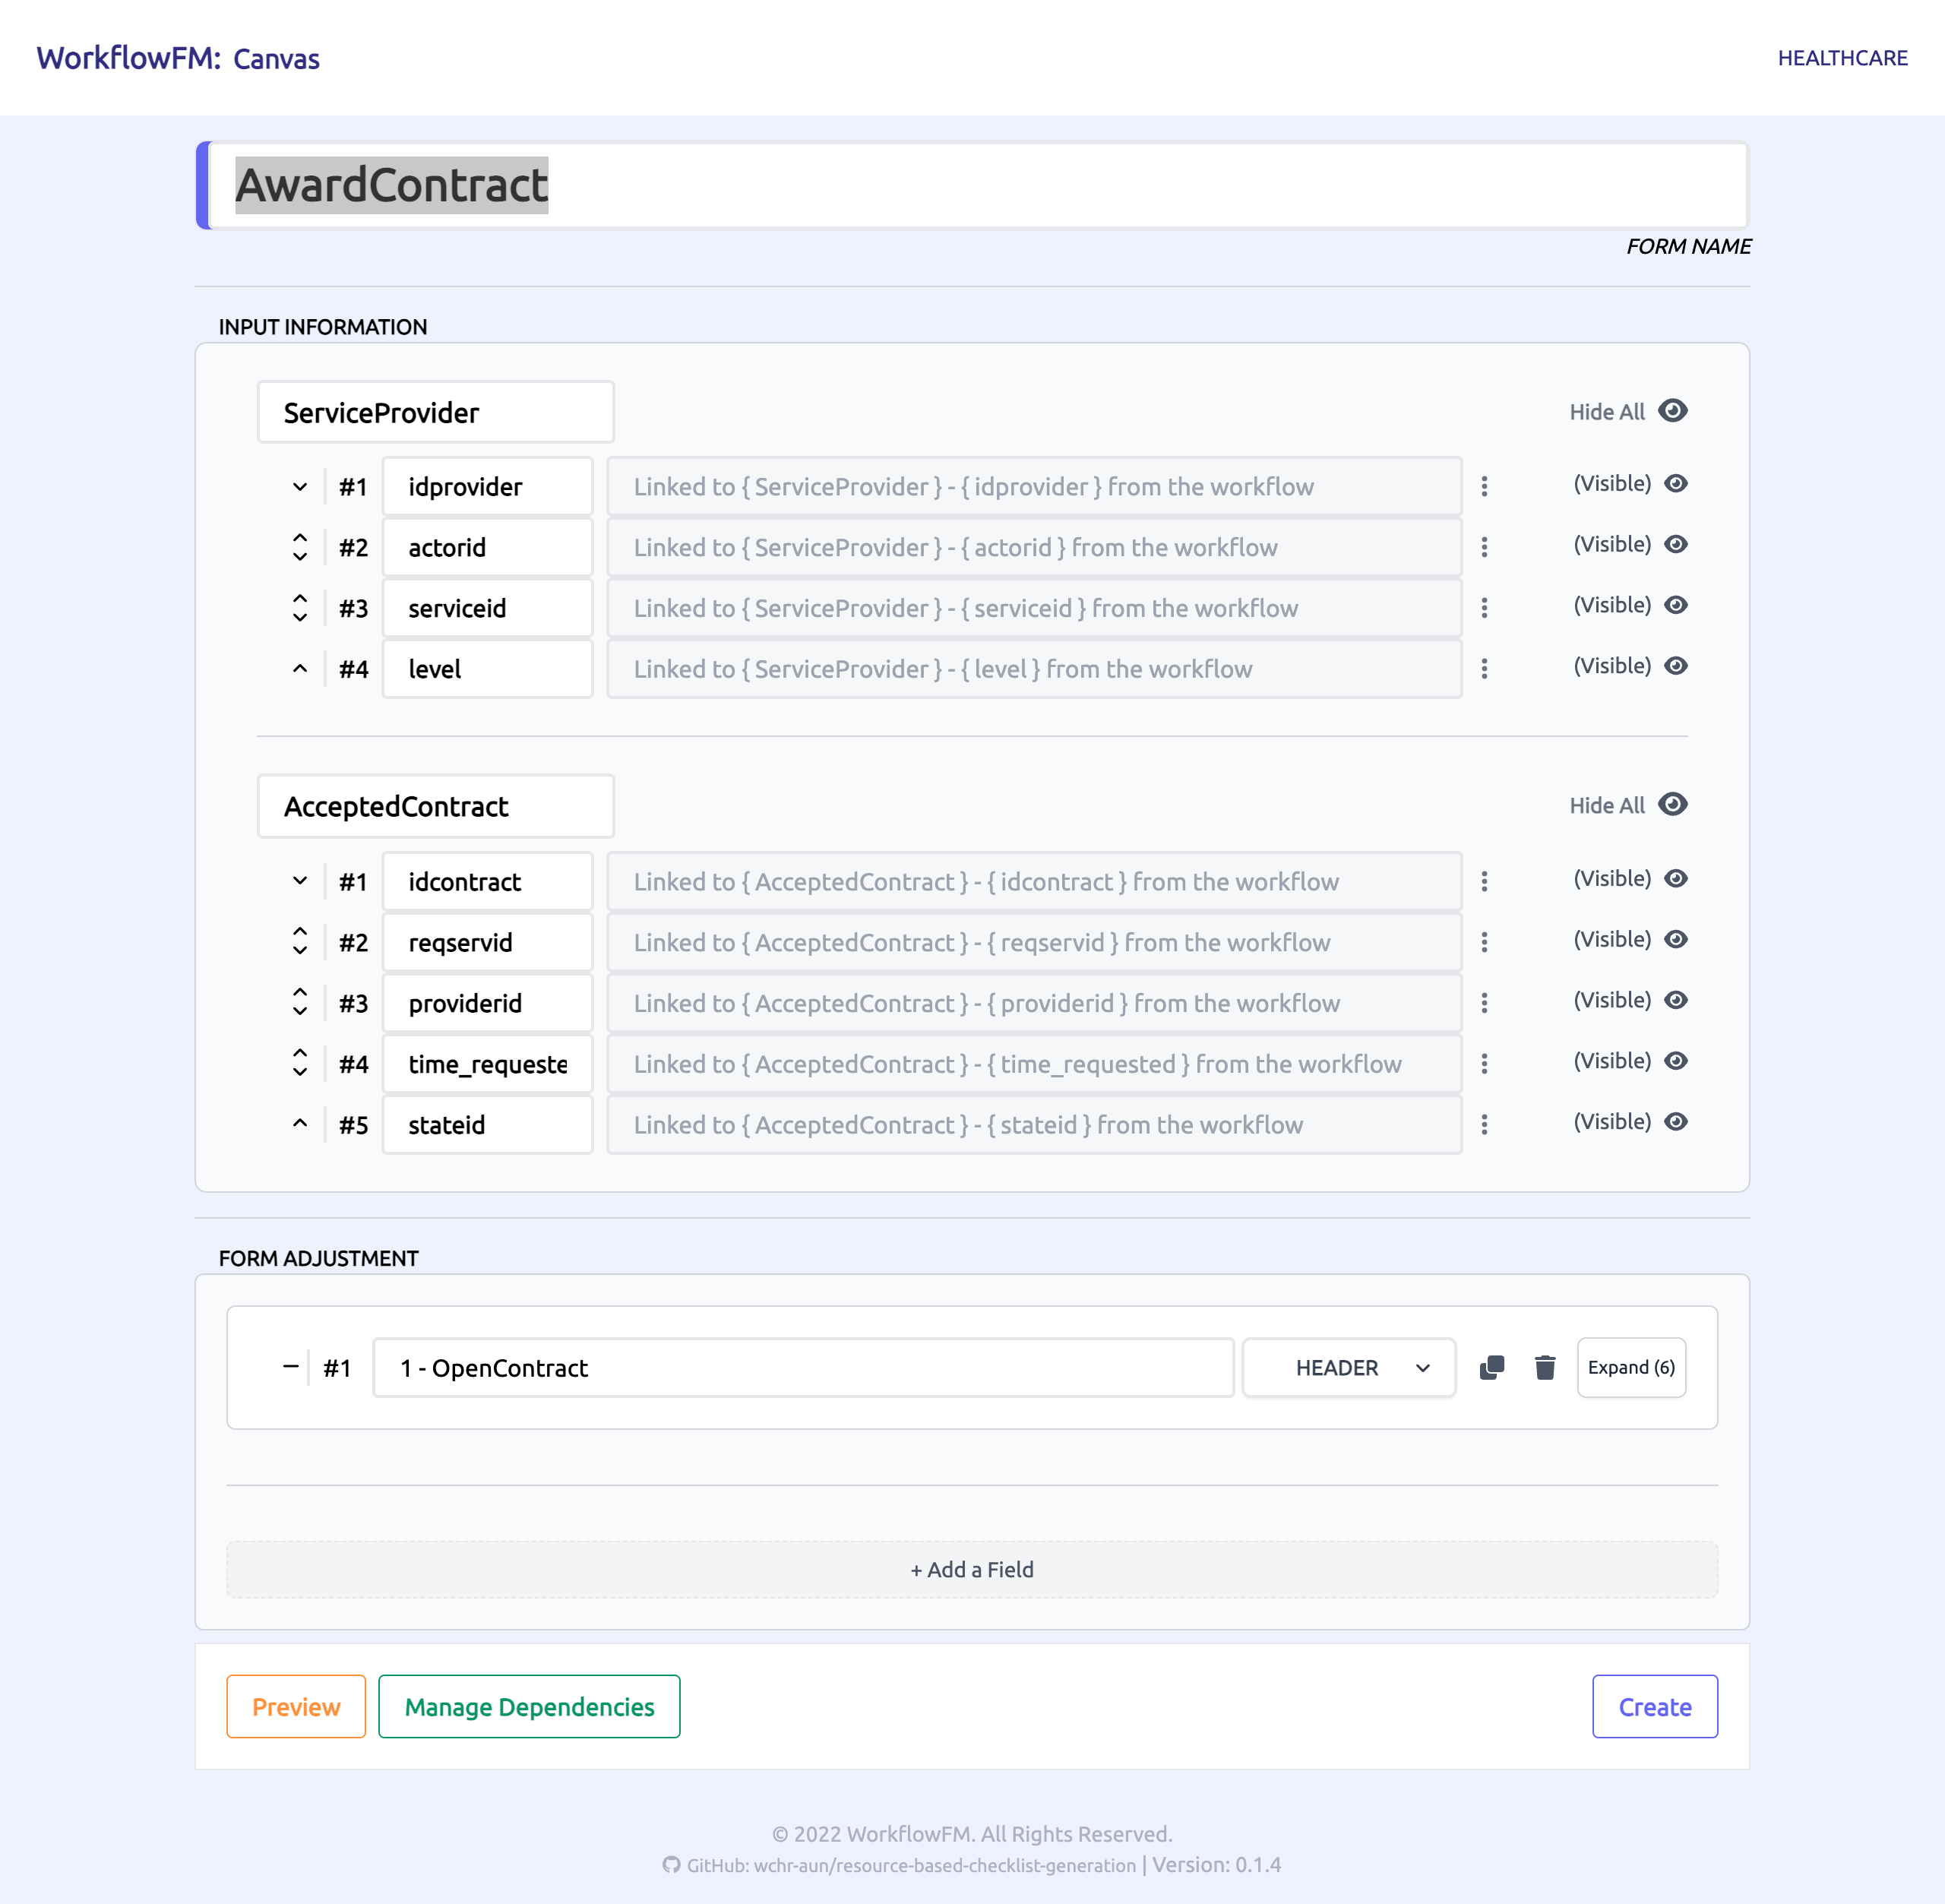
\includegraphics[width=0.9\linewidth]{overleaf/images/screens/canvas_screen.png}
  \caption{Canvas Screen}
  \label{fig:canvas_screen}
\end{minipage}%
\begin{minipage}{.5\textwidth}
  \centering
  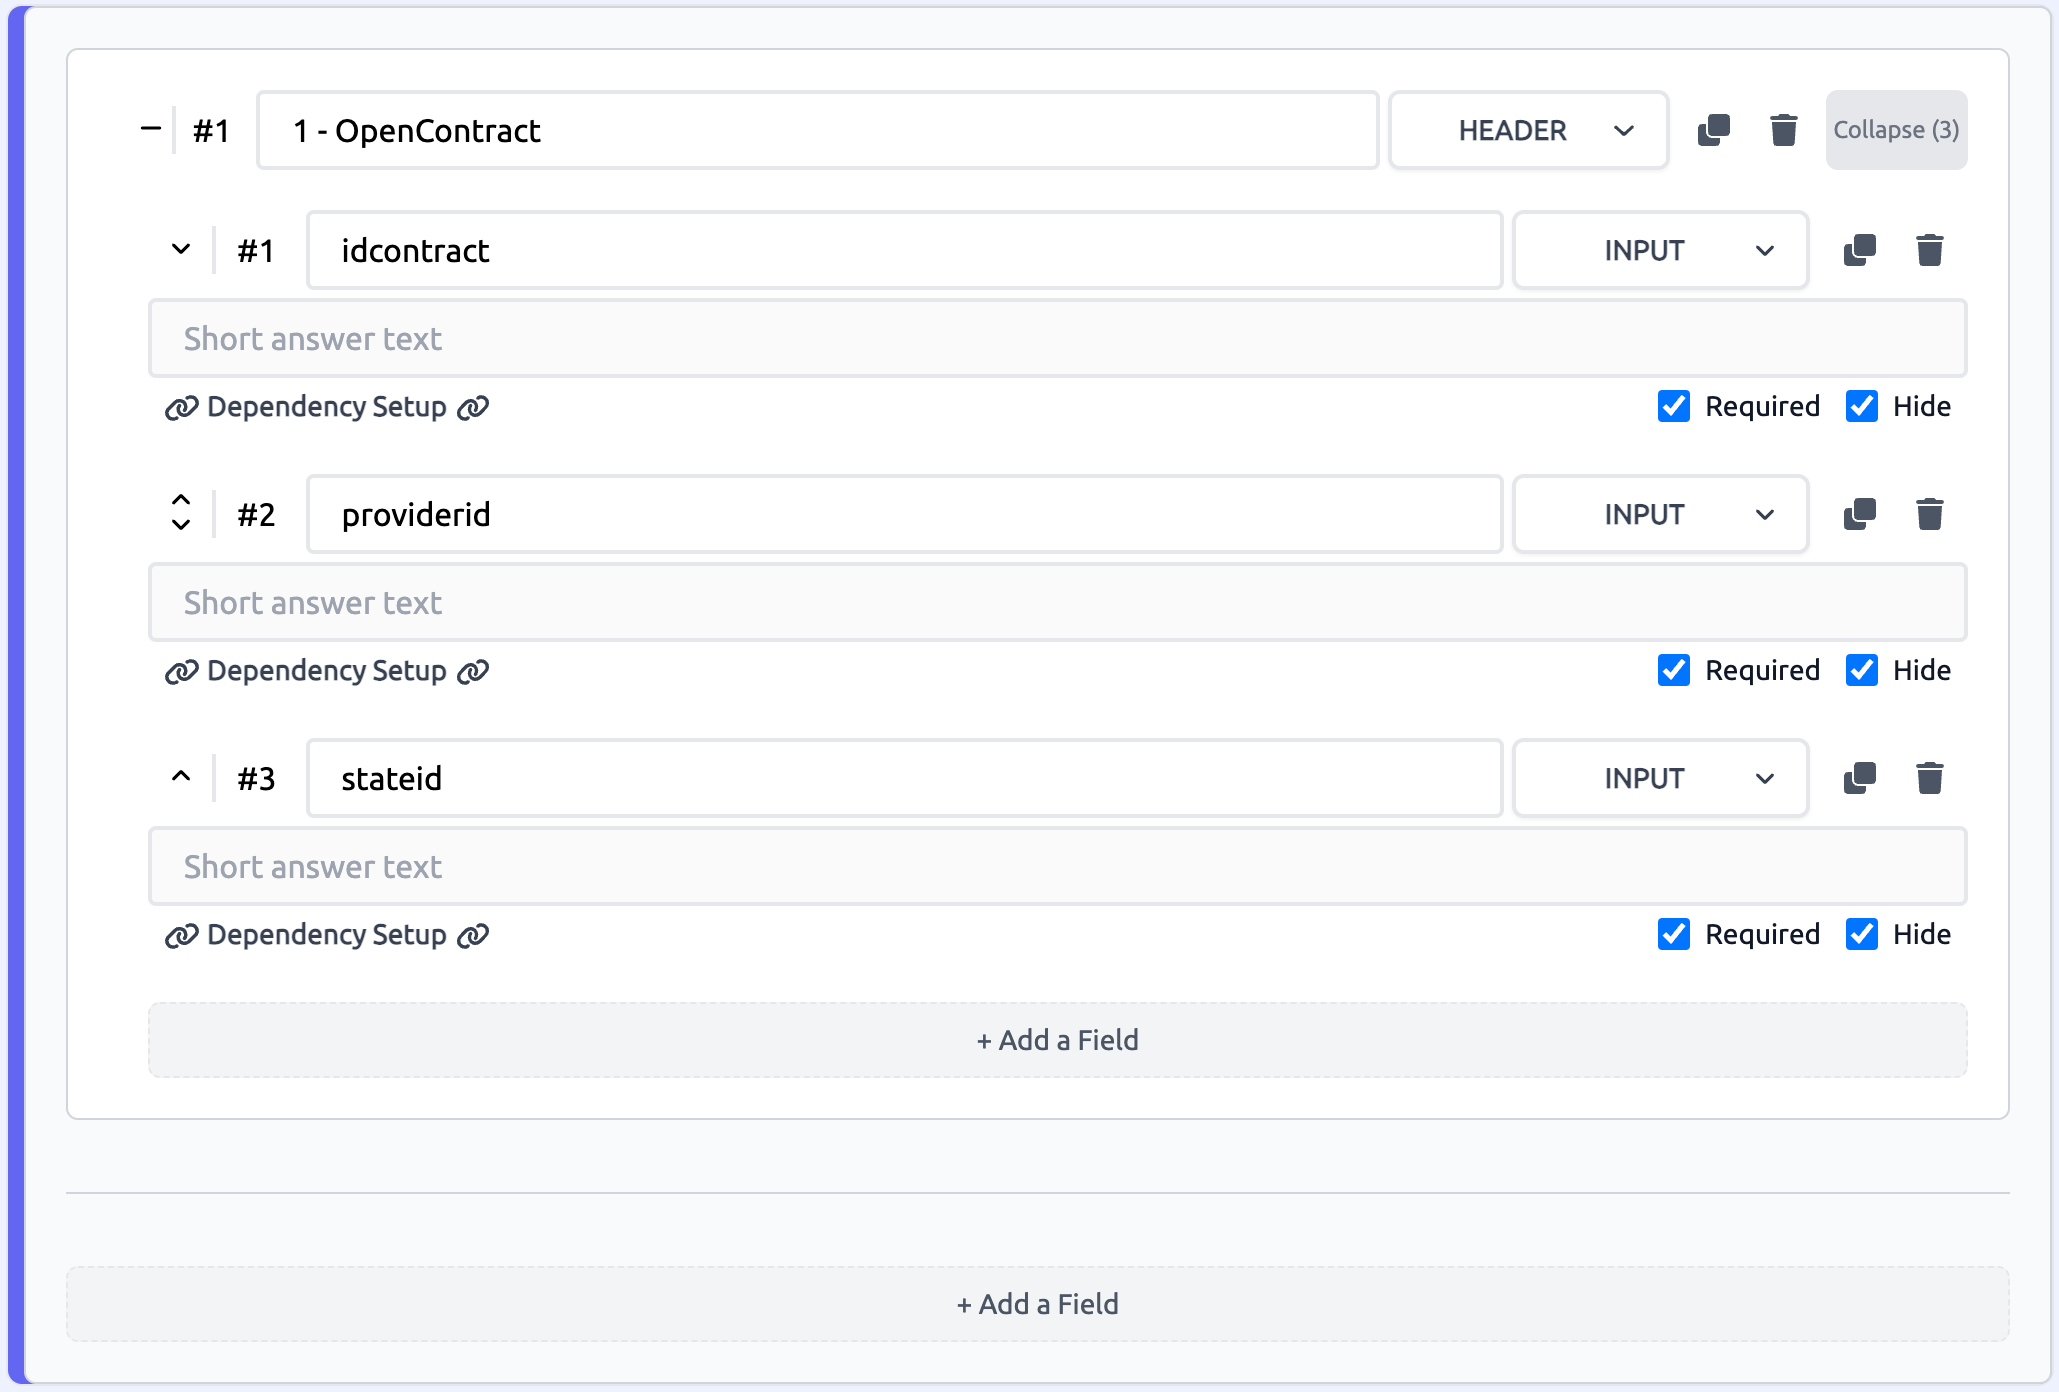
\includegraphics[width=0.9\linewidth]{overleaf/images/screens/form_section.png}
  \caption{Form Section}
  \label{fig:form_section}
\end{minipage}
\end{figure}


% Additional parts of the input infromation section
Additional to the input information section, new input information fields can be added through either ``Query more information using this field" or ``Get suggested query input information" options inside the vertical ellipsis icon (\vdots) in Figure \ref{fig:input_information_section}. This is the \textbf{Input Information Query} function. Selecting ``Get suggested query input information" will call the \textbf{Query Suggestion} function and display all the suggested fields, as shown in \ref{fig:query_suggestion}. Both the \textbf{Input Information Query} function and the \textbf{Query Suggestion} functionalities will be further elaborated in section \ref{backend_dependency}




\begin{figure}[ht!]
\centering
\begin{minipage}{.5\textwidth}
  \centering
  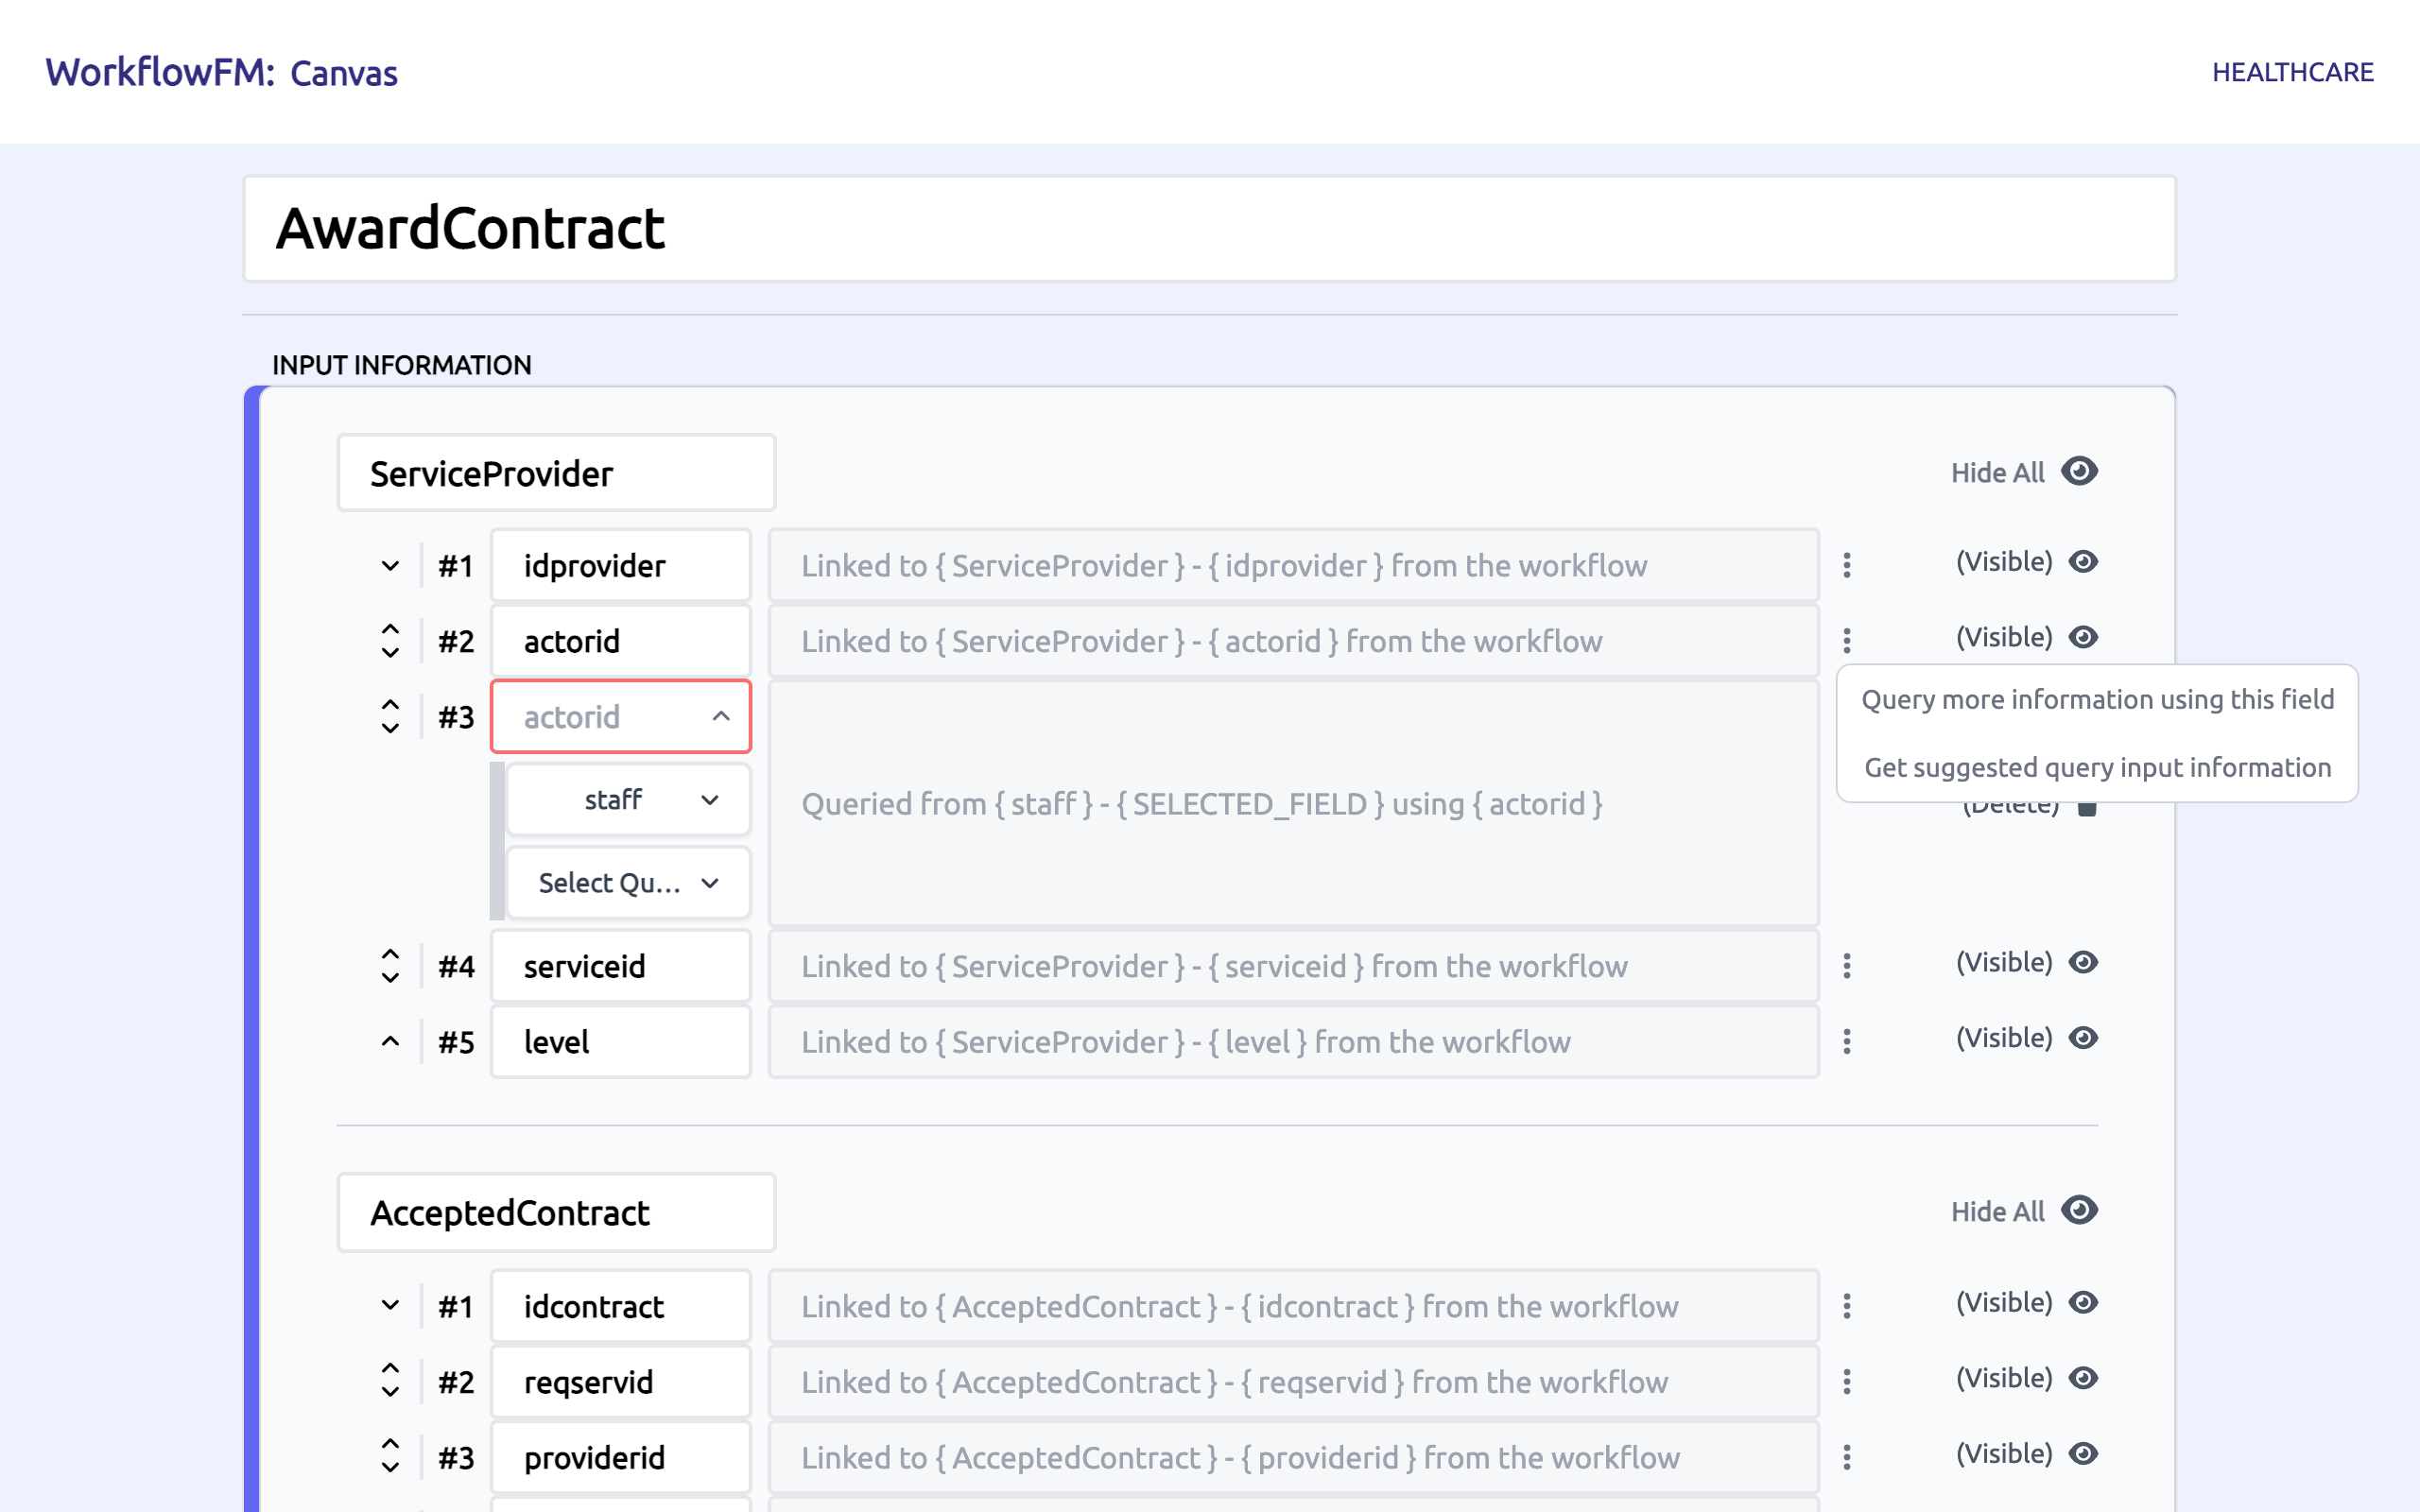
\includegraphics[width=0.9\linewidth]{overleaf/images/screens/input_information_section.png}
  \caption{Input Information Section}
  \label{fig:input_information_section}
\end{minipage}%
\begin{minipage}{.5\textwidth}
  \centering
  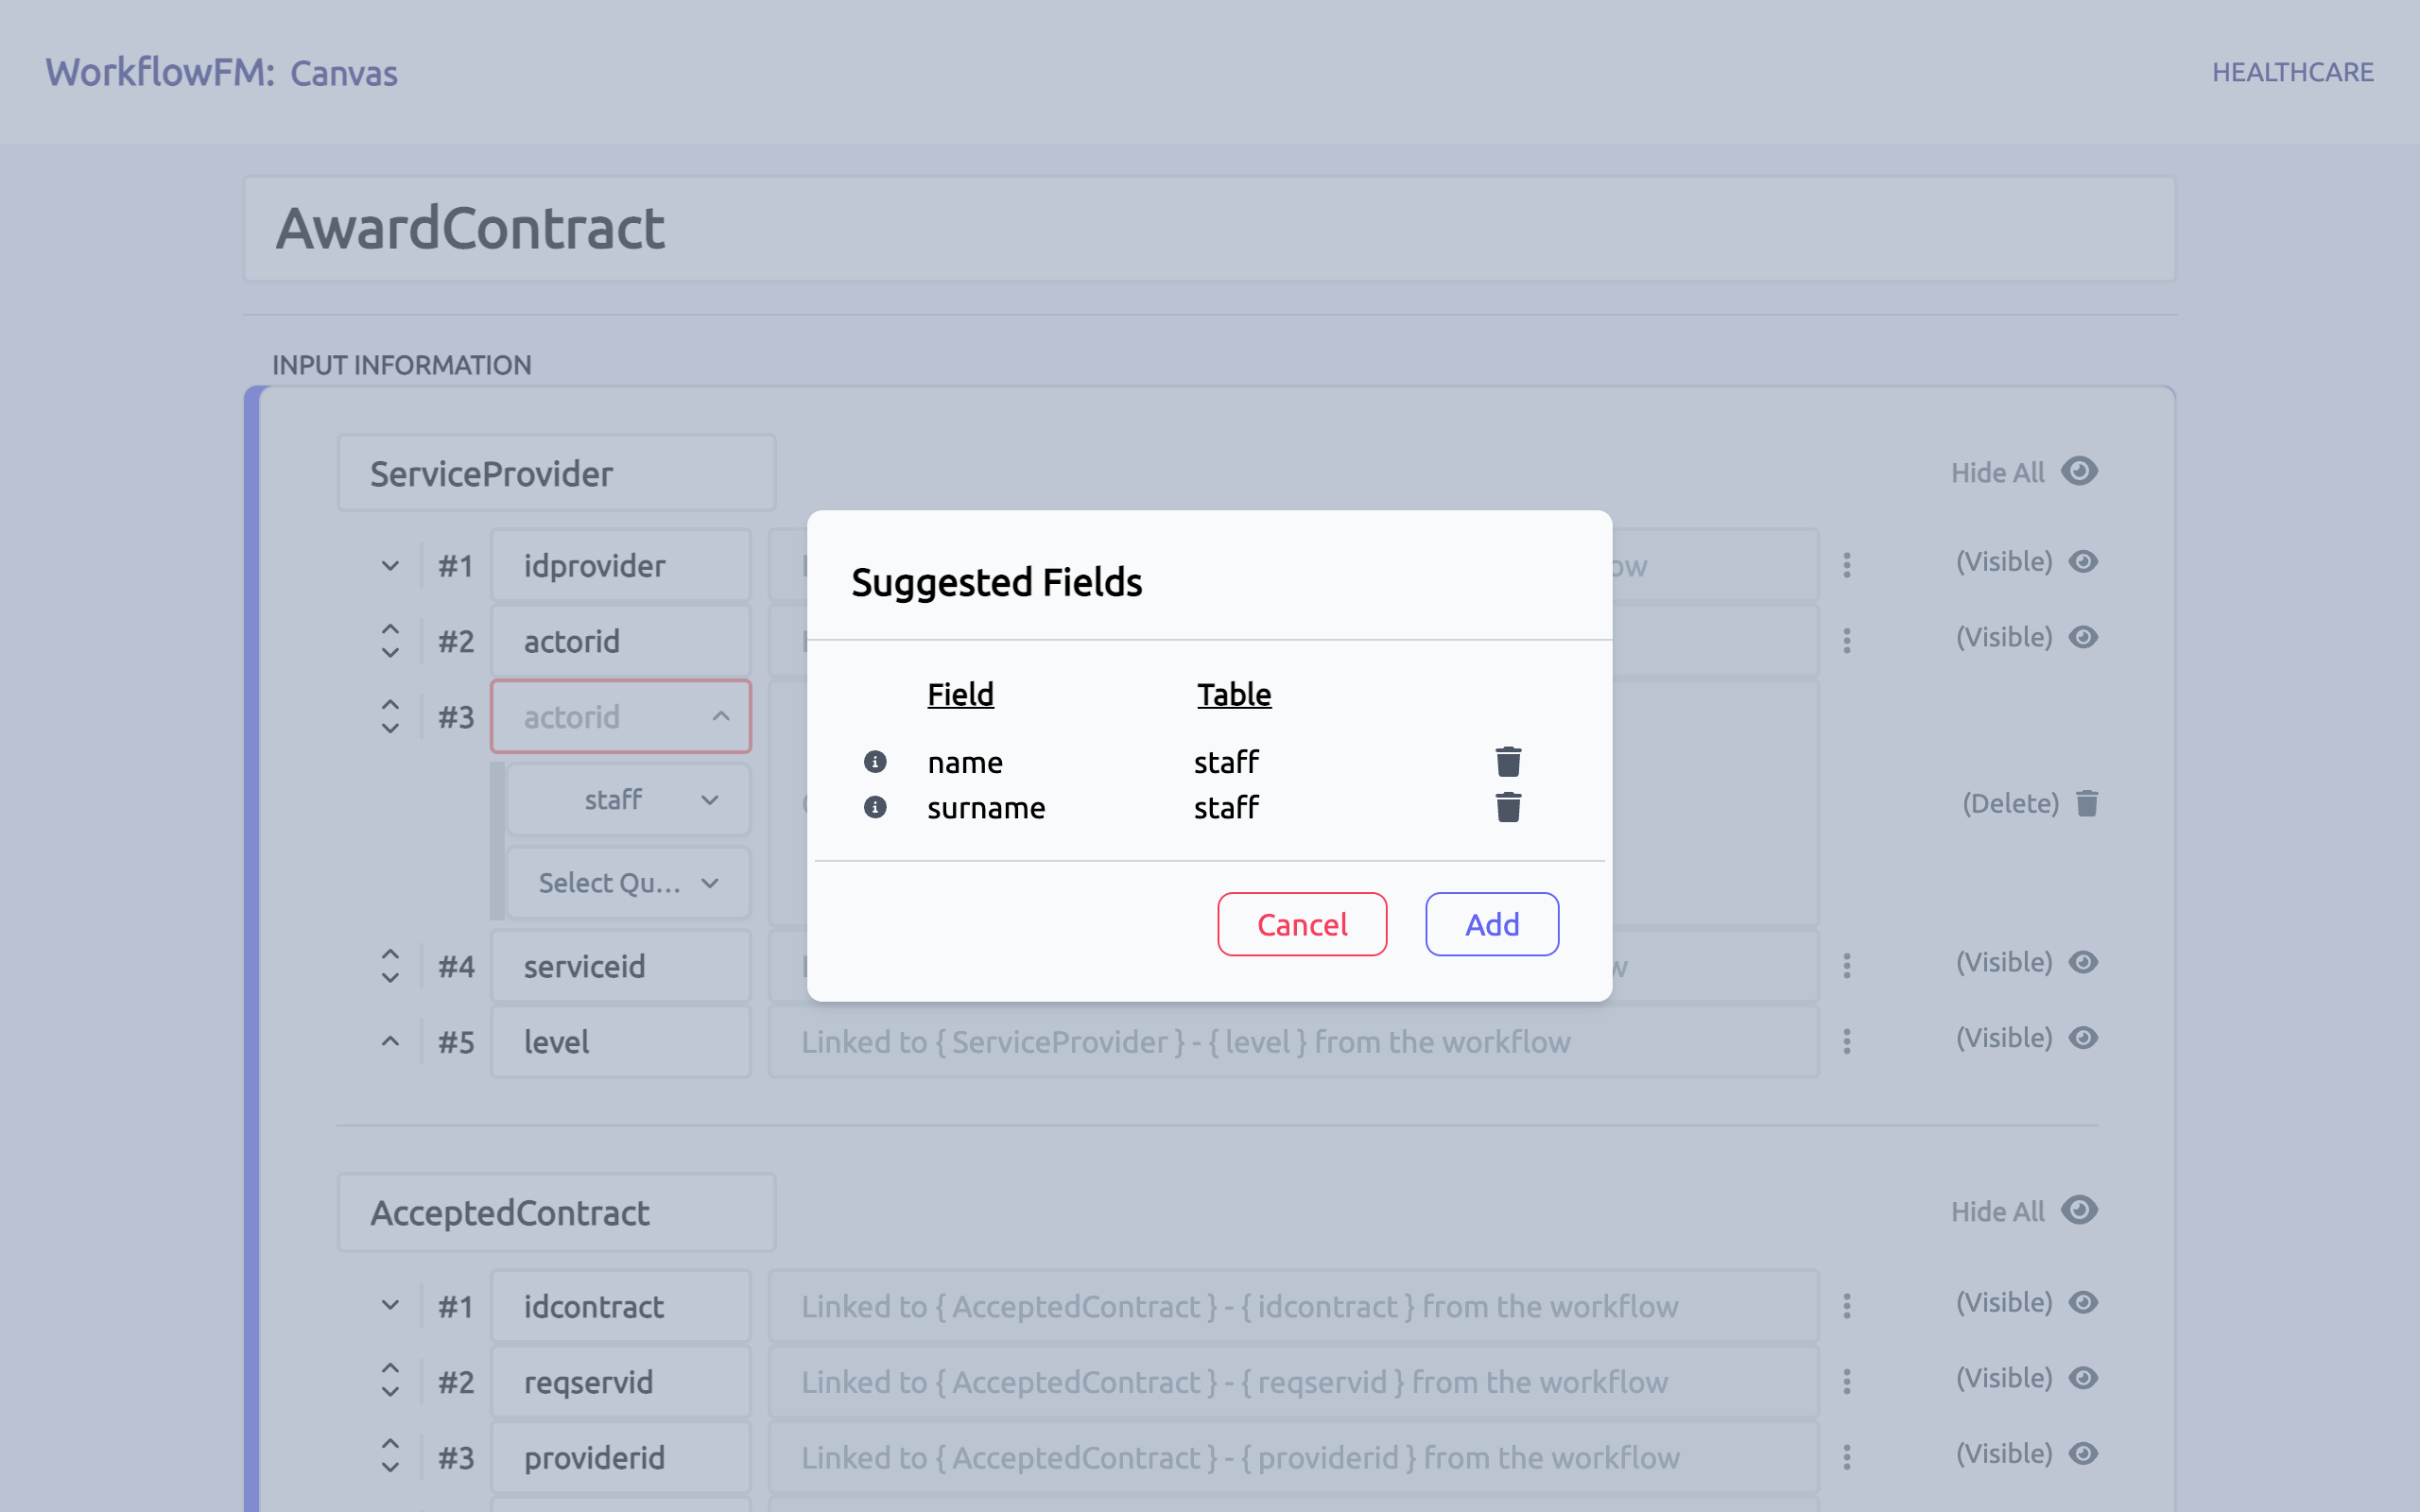
\includegraphics[width=0.9\linewidth]{overleaf/images/screens/query_suggestion.png}
  \caption{Query Suggestion Popup}
  \label{fig:query_suggestion}
\end{minipage}
\end{figure}


% \begin{figure}[ht!]
%     \centering
%     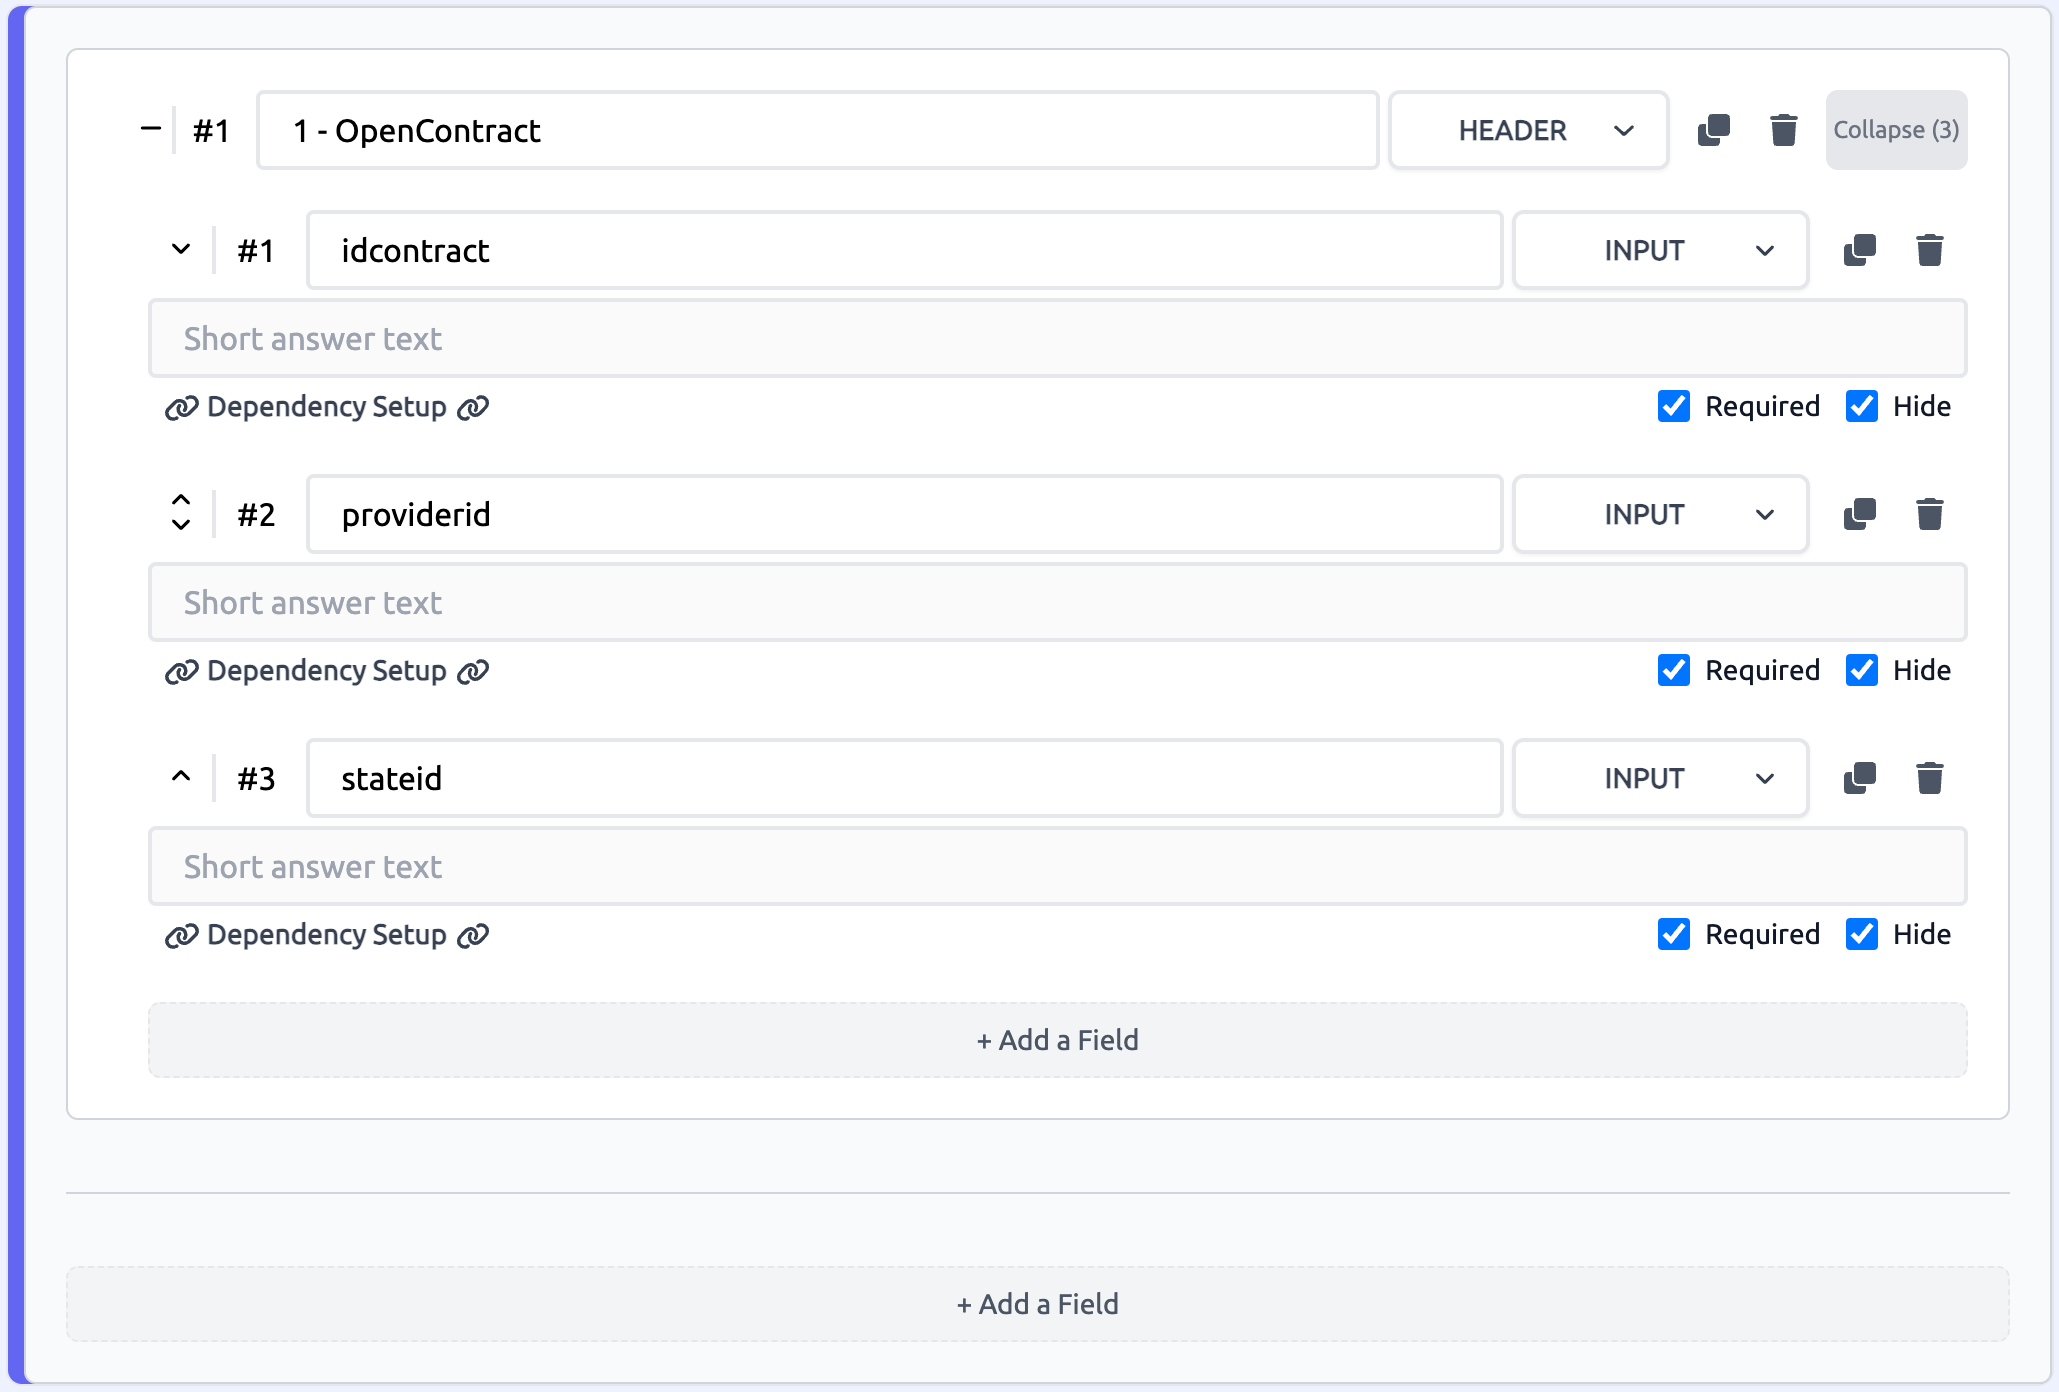
\includegraphics[width=0.5\textwidth]{overleaf/images/screens/form_section.png}
%     \caption{Form Section}
%     \label{fig:form_section}
% \end{figure}


\subsubsection{Dependencies Management Popups}
\label{im:depend_manage_pop}

Dependencies management popups can be accessed through the dependency setup button under each form component or the manage dependencies button at the bottom of the canvas screen (\ref{im:canvas_screen}). Accessing the dependency setup button will bring users to the component's dependencies setup. This popup is dedicated to each component, as shown in Figure \ref{fig:edit_dependencies_2}. On the other hand, the manage dependencies button will lead users to the all components' dependencies management popup, as seen in Figure \ref{fig:edit_dependencies}. Setting up input and output dependencies in these popups is part of the \textbf{Dependency Linking} function.

\begin{figure}[ht!]
\centering
\begin{minipage}{.5\textwidth}
  \centering
  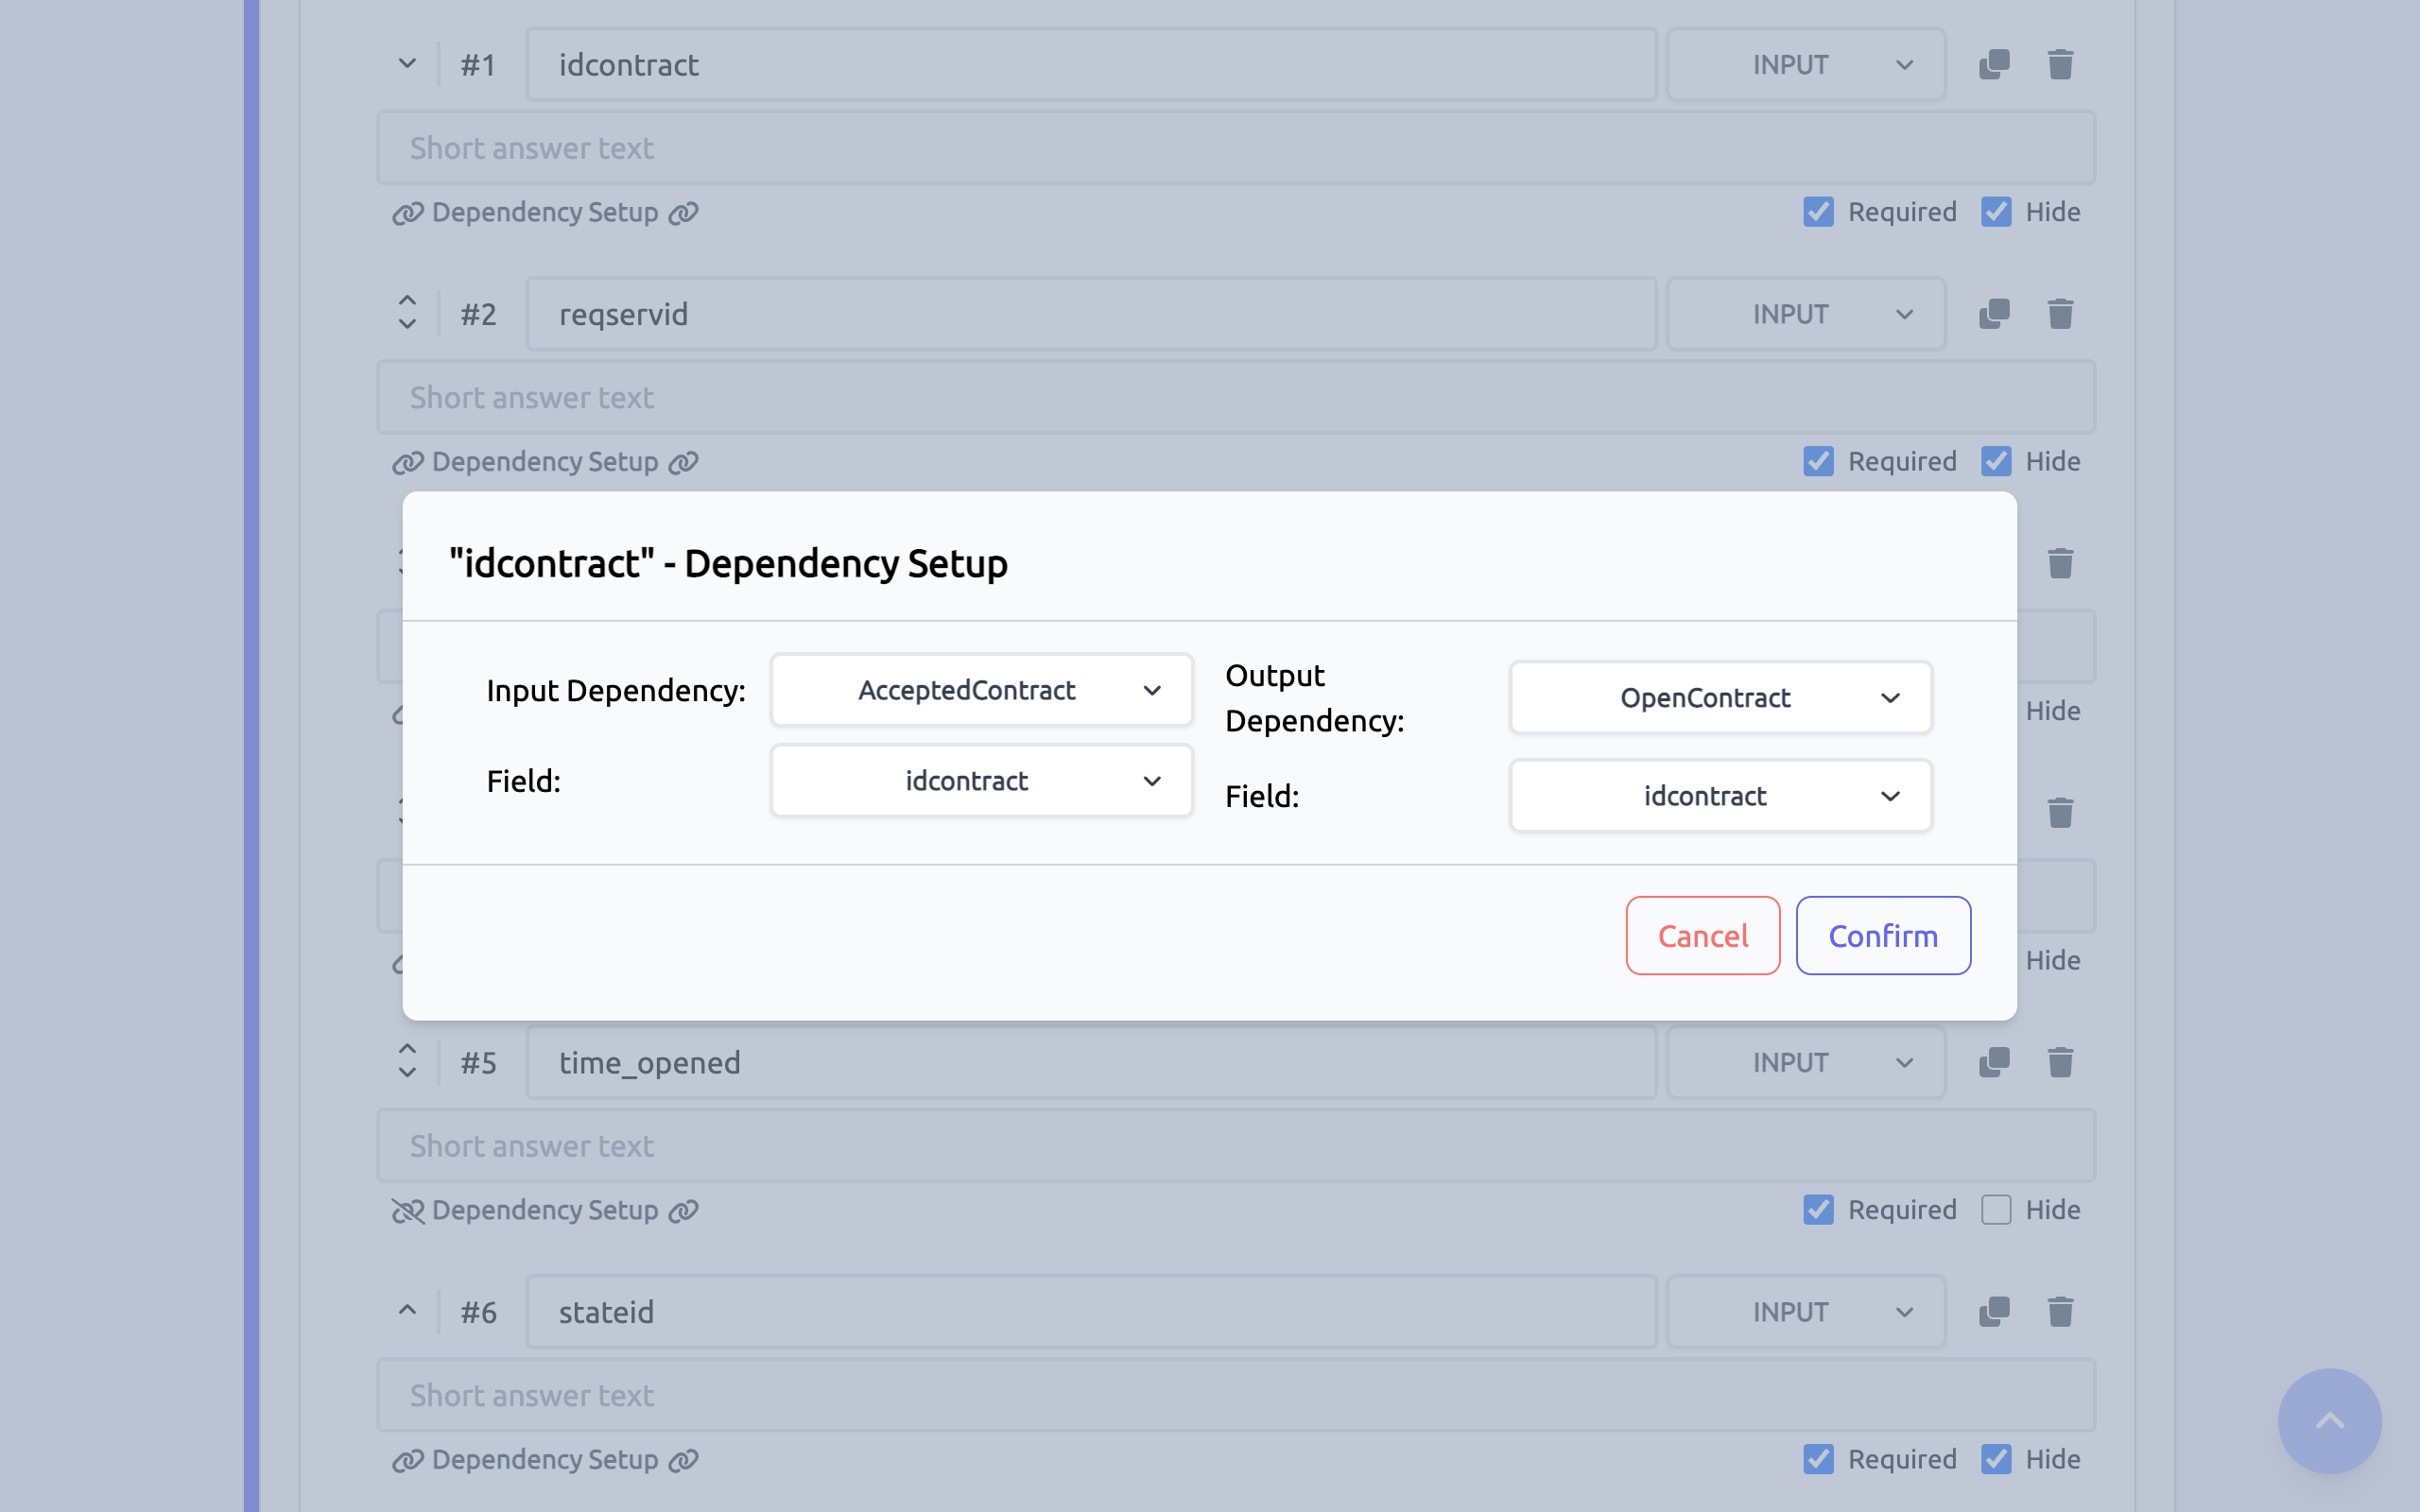
\includegraphics[width=0.9\linewidth]{overleaf/images/screens/edit_dependencies_2.png}
  \caption{Dependency Setup}
  \label{fig:edit_dependencies_2}
\end{minipage}%
\begin{minipage}{.5\textwidth}
  \centering
  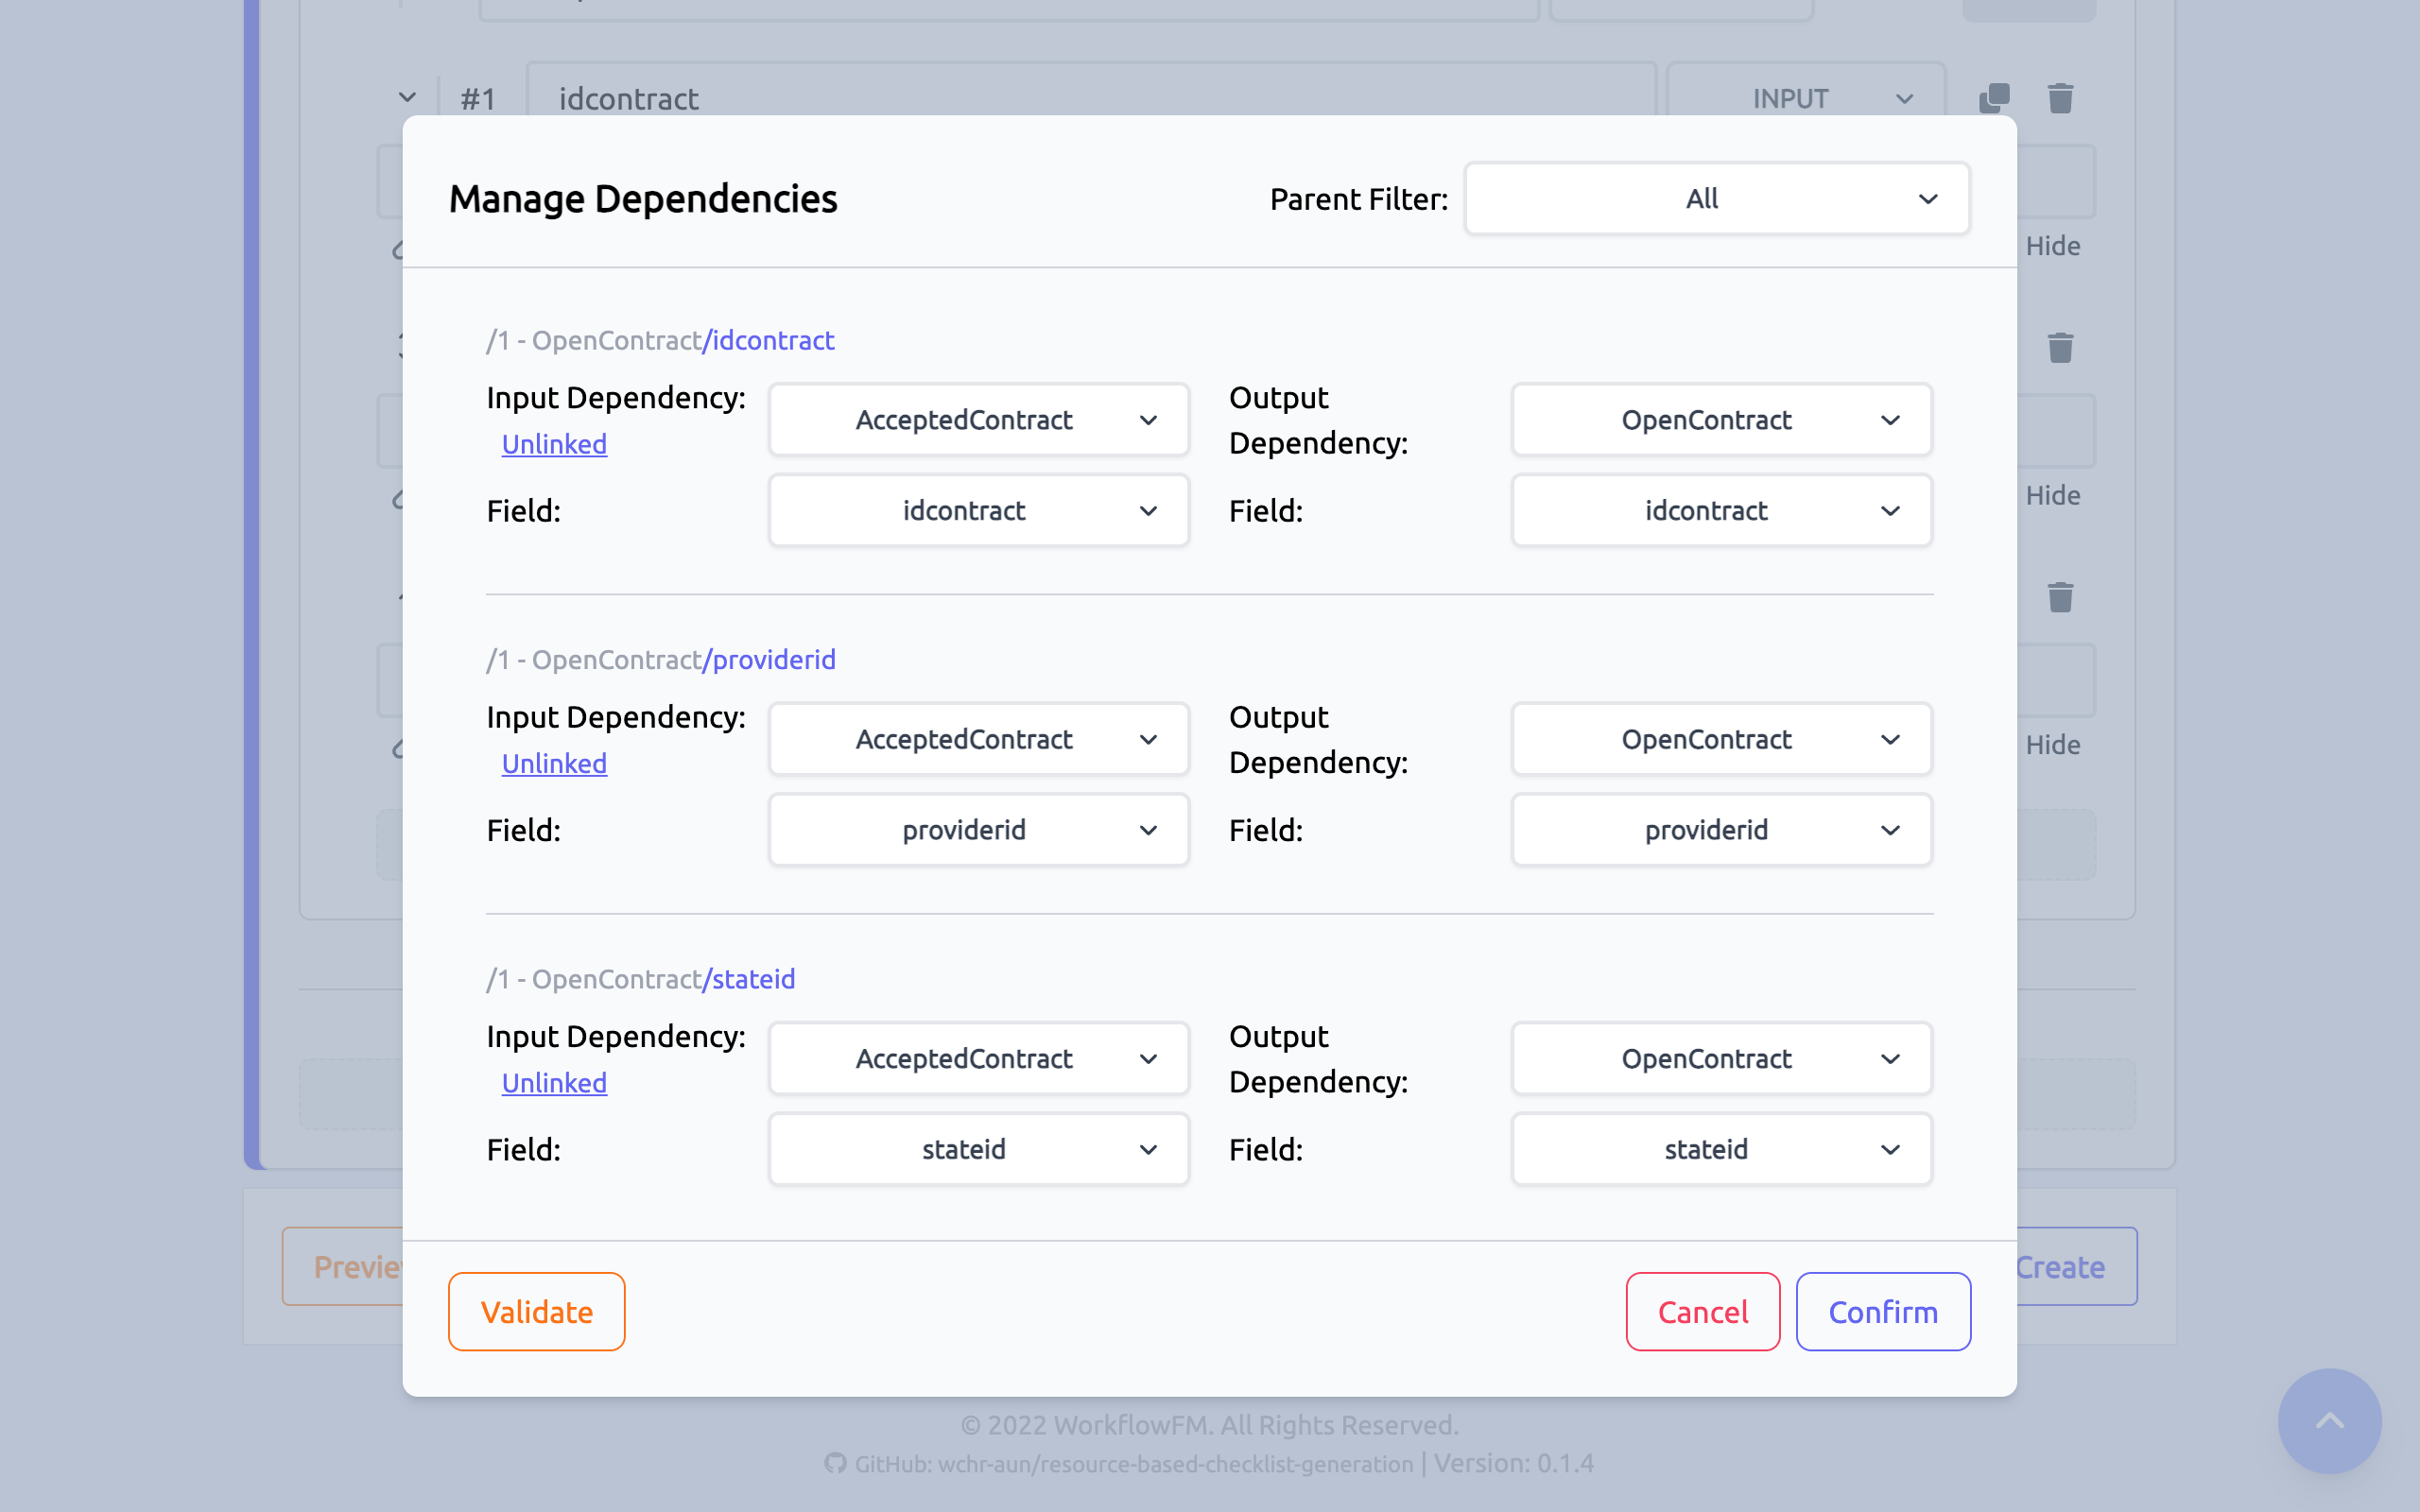
\includegraphics[width=0.9\linewidth]{overleaf/images/screens/edit_dependencies.png}
  \caption{Dependencies Management}
  \label{fig:edit_dependencies}
\end{minipage}
\end{figure}

\subsubsection{Preview Screen}
\label{im:preview_screen}

Preview screen is the screen that allows users to visualise how the template would look like when it is created. This screen can be accessed through the preview button in the canvas screen (\ref{im:canvas_screen}).

\begin{figure}[ht!]
    \centering
    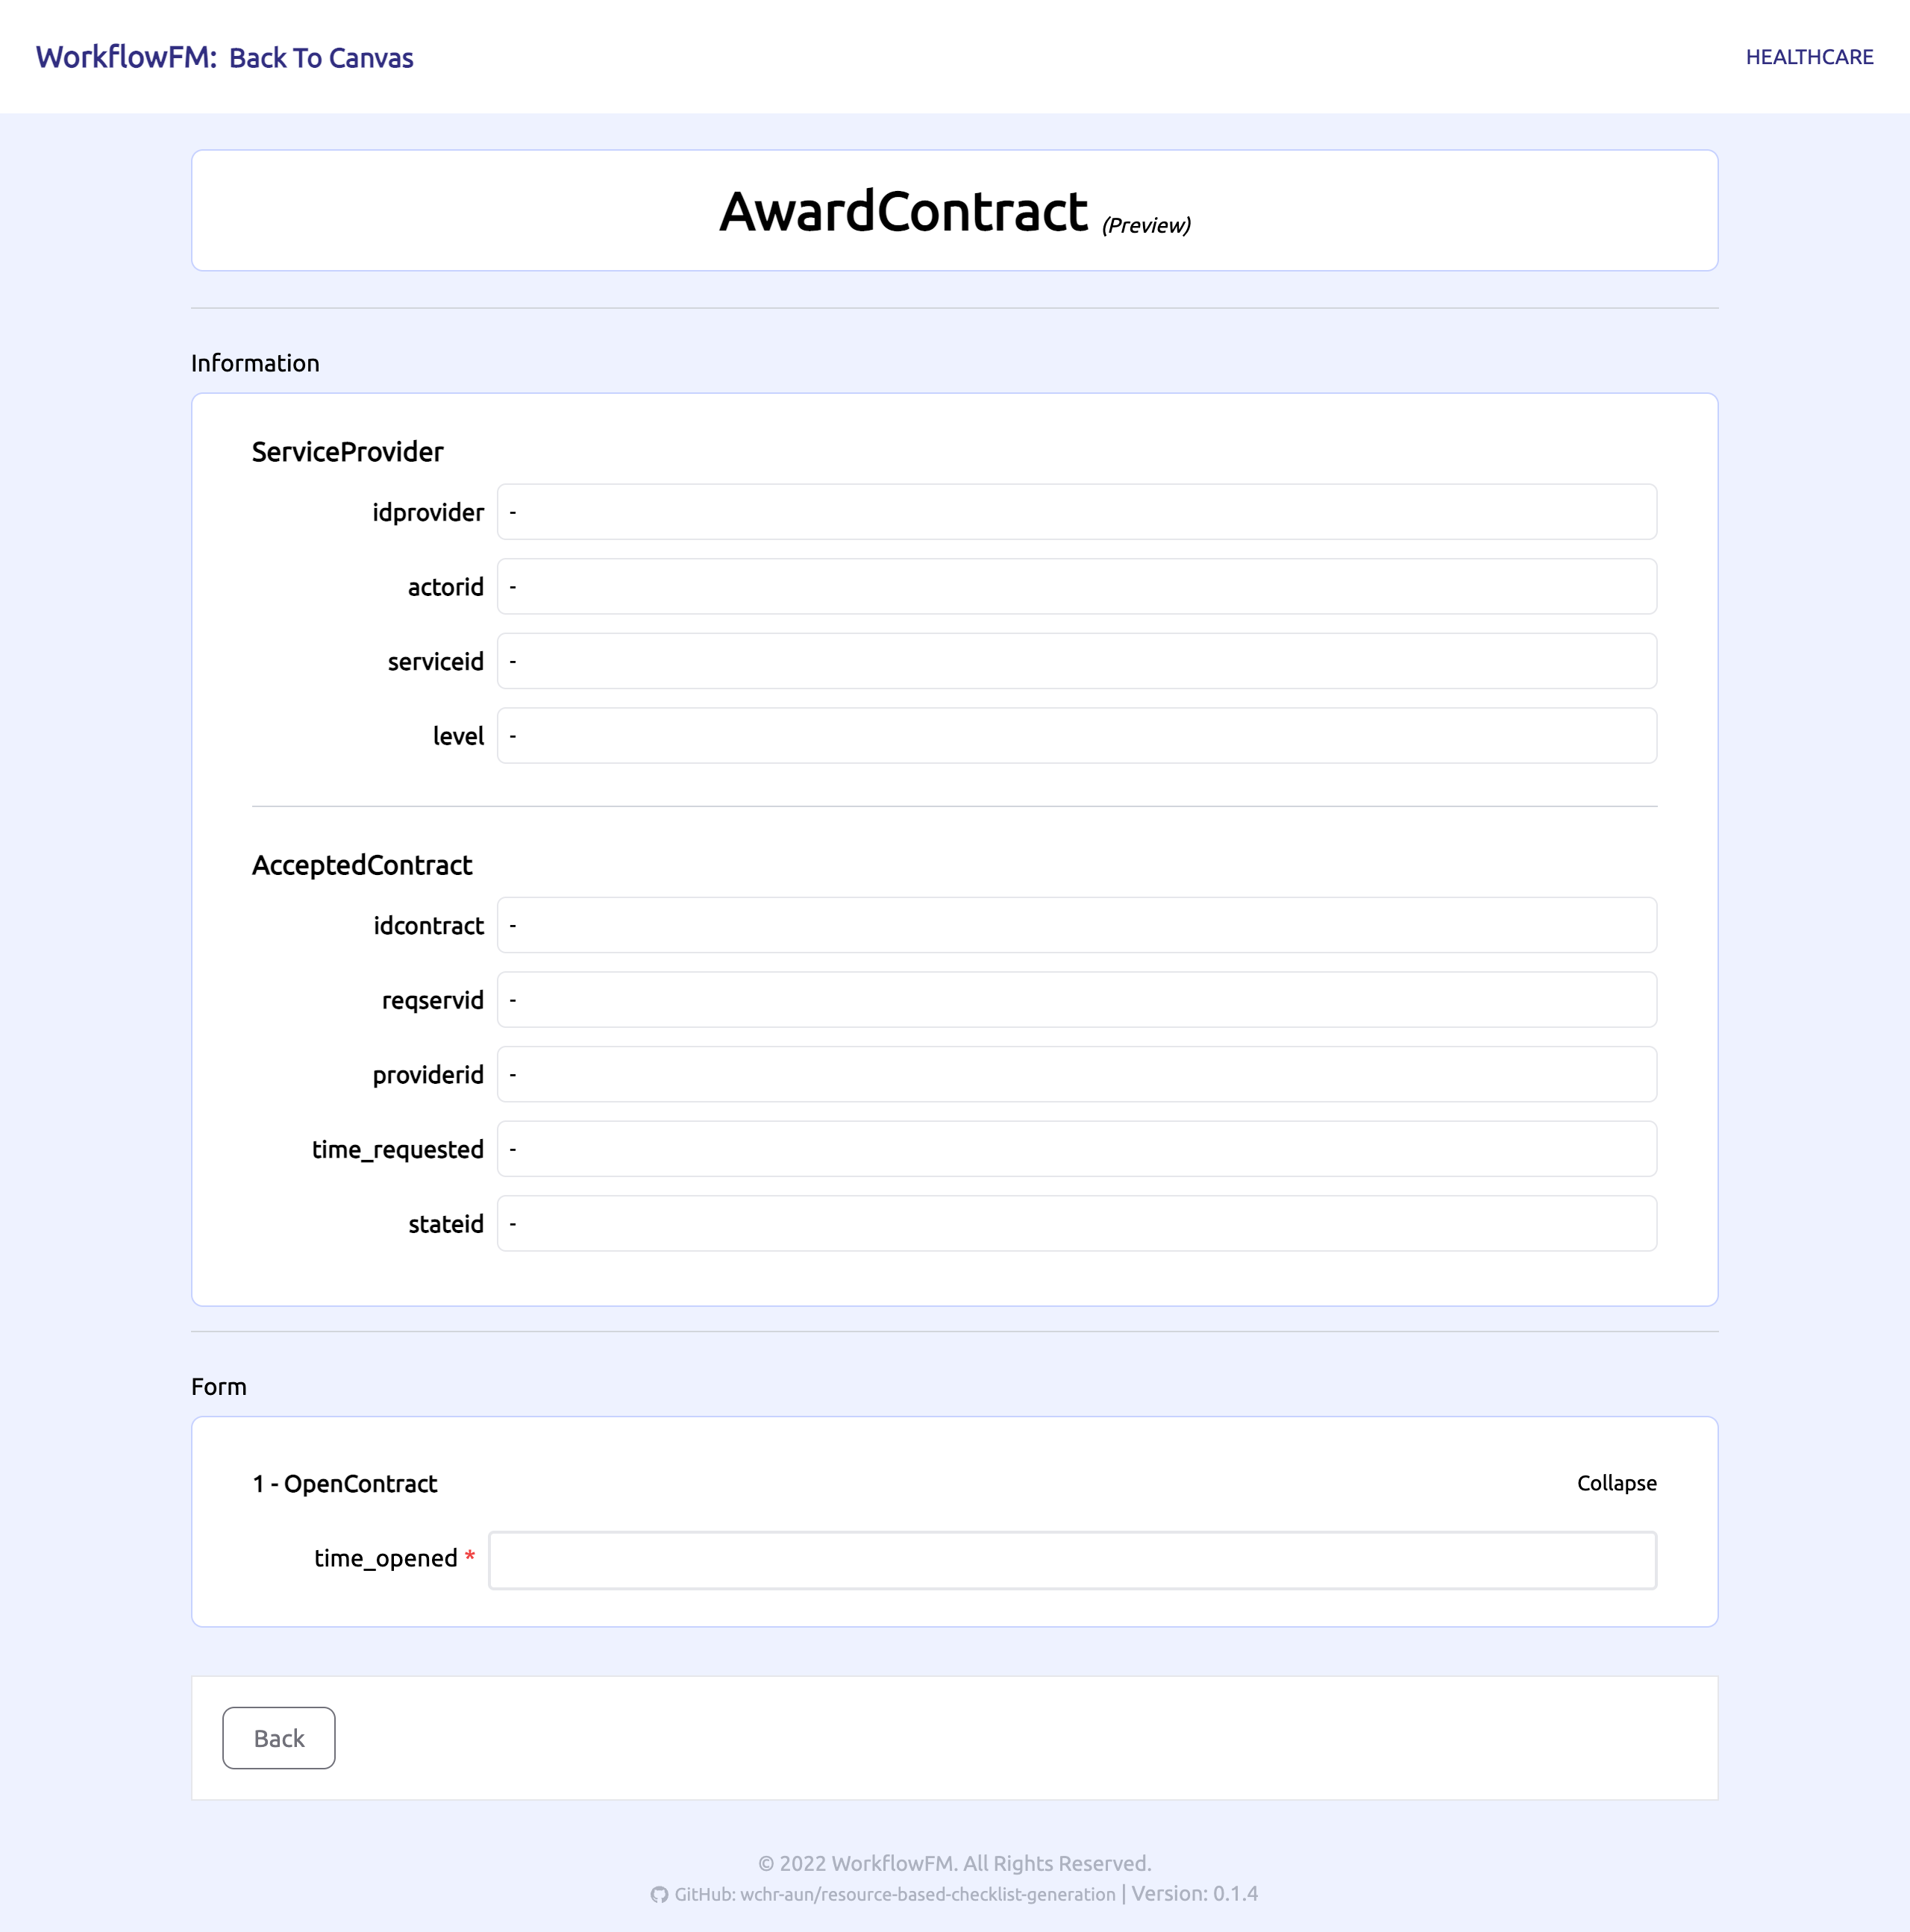
\includegraphics[width=0.55\textwidth]{overleaf/images/screens/preview_screen.png}
    \caption{Preview Screen}
    \label{fig:preview_screen}
\end{figure}





\subsection{Checklist}
\label{im:view_checklist}

As discussed in the software's structure section \ref{fig:software_structure}, this component only has one dynamic screen which displays differently based on the selected template from the list on the main screen. Being able to view a saved template is part of the \textbf{View Checklist Template} function.

\begin{figure}[ht!]
    \centering
    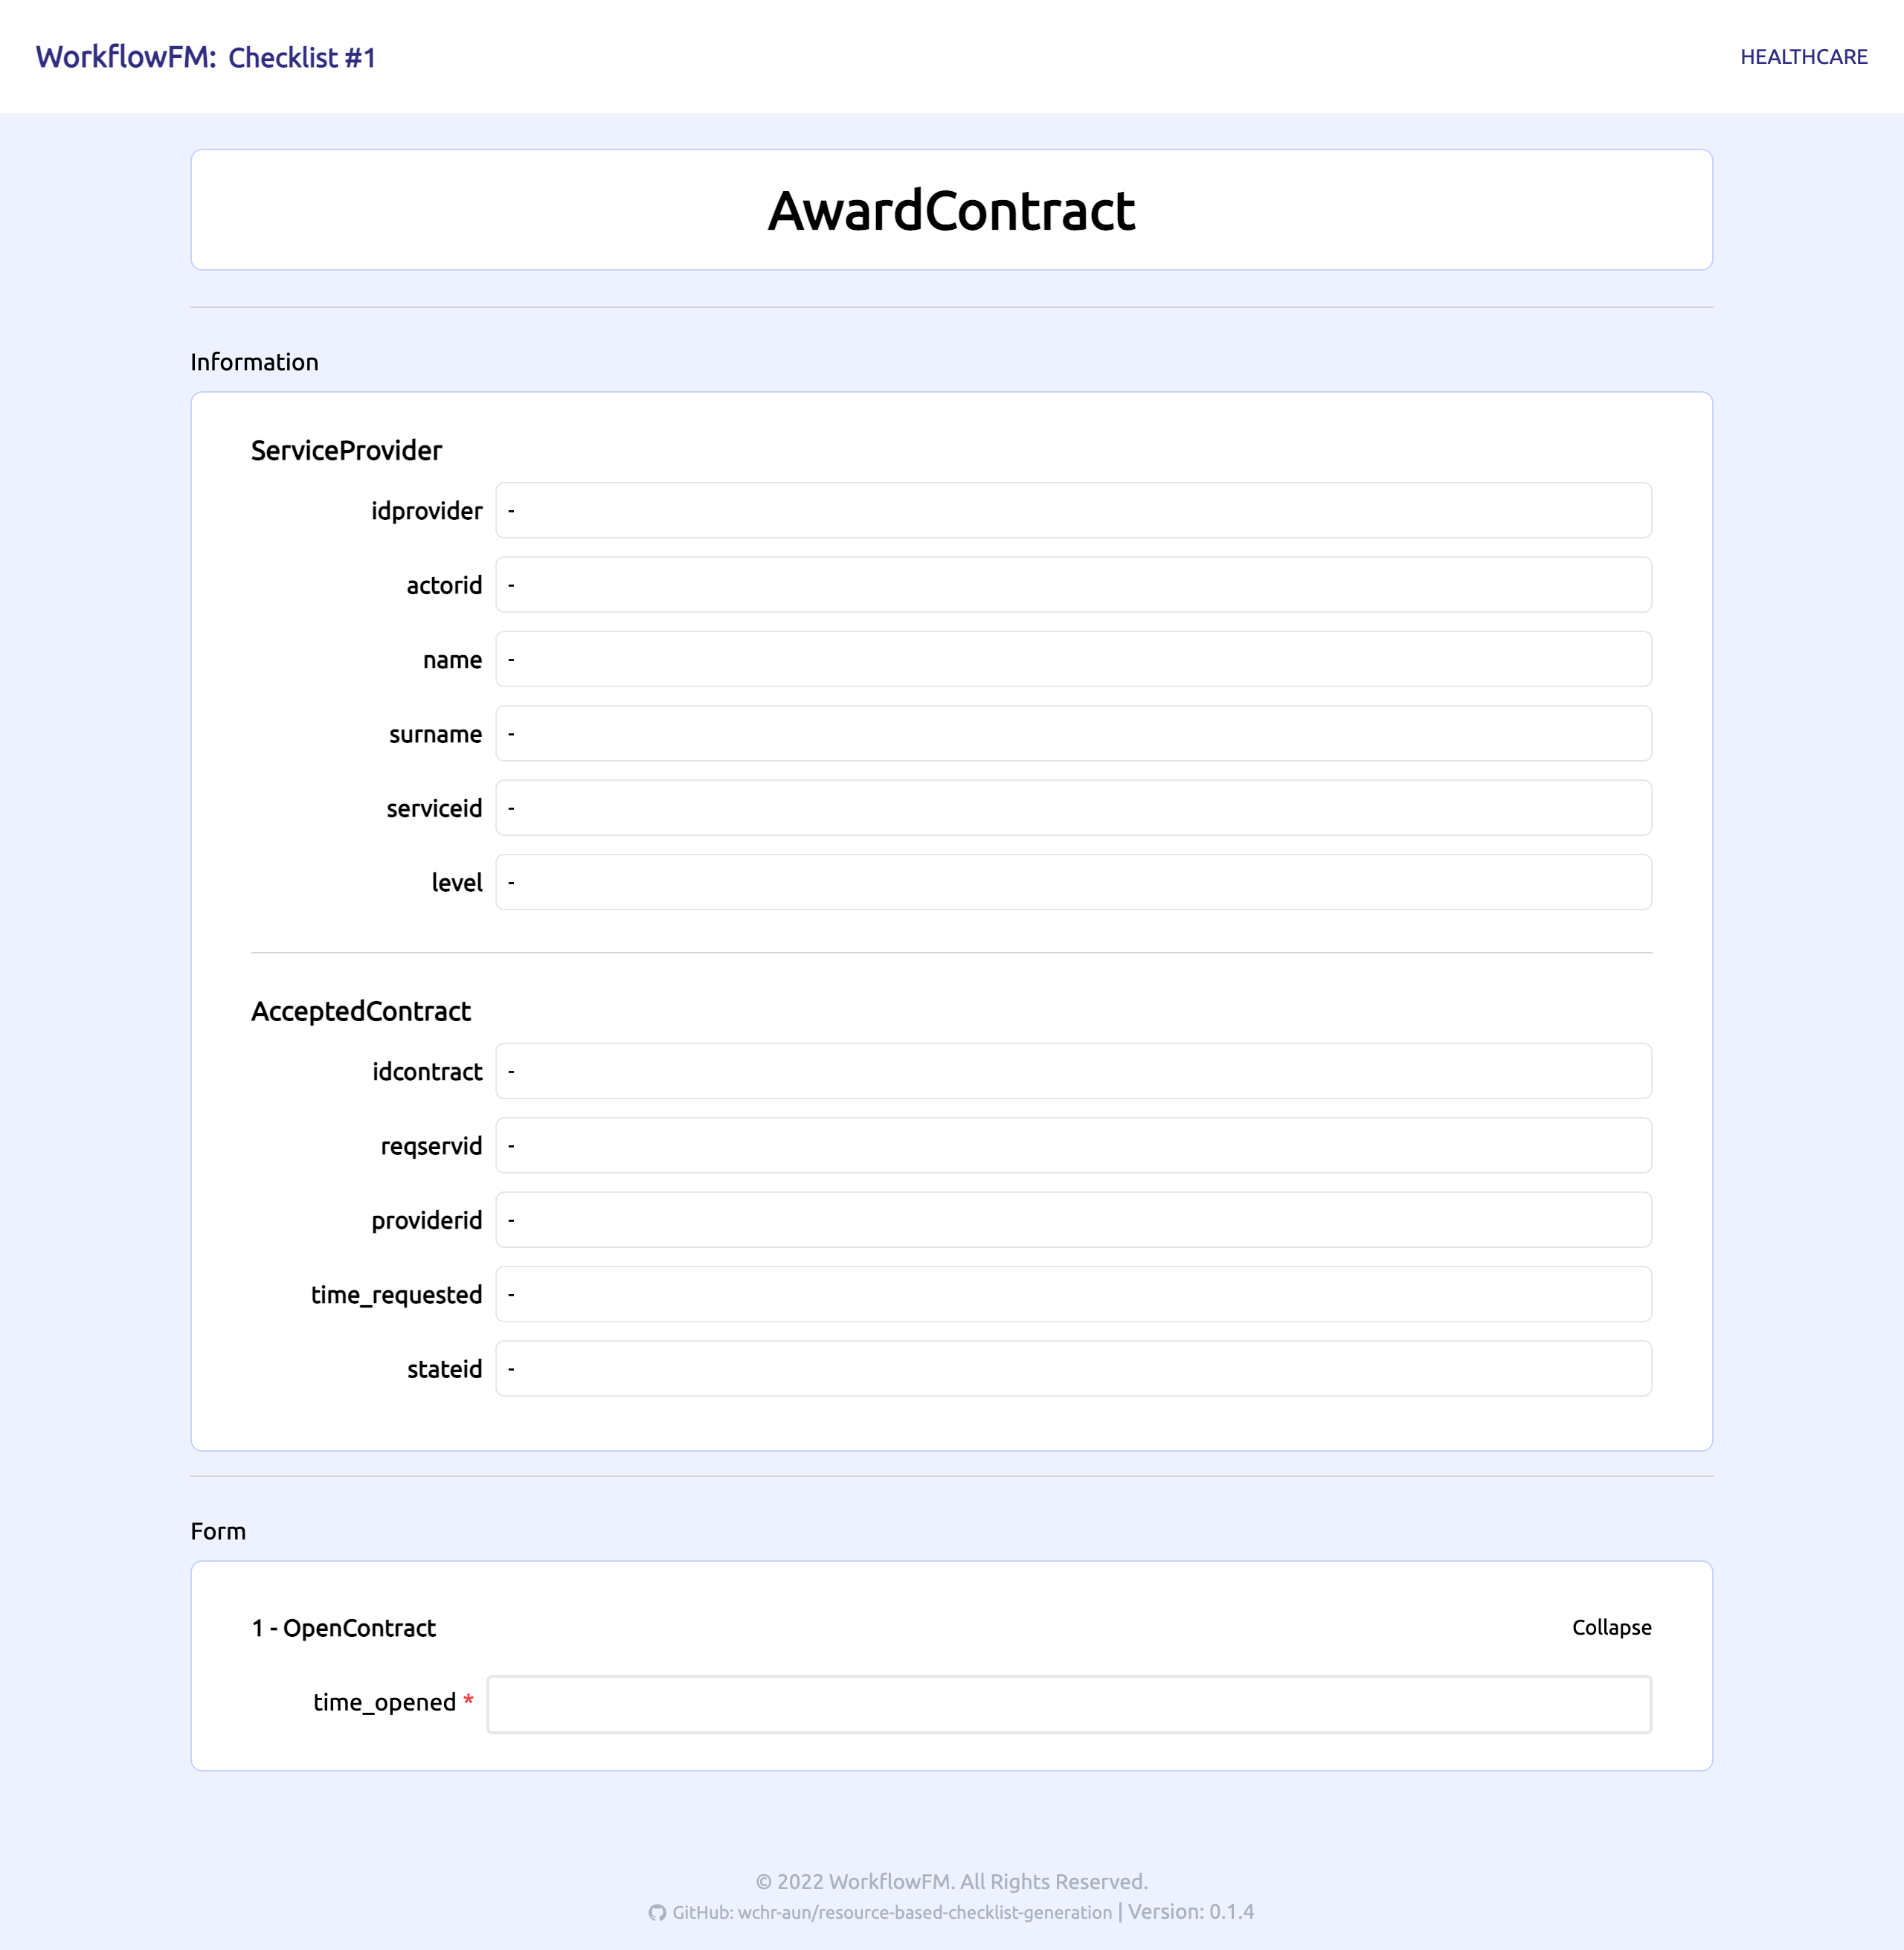
\includegraphics[width=0.55\textwidth]{overleaf/images/screens/view_checklist_screen.png}
    \caption{Checklist Screen}
    \label{fig:view_checklist_screen}
\end{figure}

\section{Backend}

asdfasd
% \subsection{Application Programming Interfaces}
% - workflow process to checklist template

% - get dependencies

% - get foreign tables/keys

% - saving template

% - retrieve finished templates


\subsection{Template}

\subsection{Dependency}
\label{backend_dependency}

\subsection{Checklist}
% \subsection{Naive Queryable Field Suggestion}
% \subsection{Naive Dependency Suggestion}


\section{Testing}


\section{Challenges}

tree structure of workflowfm's processes, doing all suggestions within sql queries, design challenges (queryable input fields)
% http4s sucks-akka-http works


\chapter{Evaluation and Results}
% results
\section{Test Scenario}

\section{Questionnaire}


\section{Unit Testing}


\chapter{Conclusions and Remarks}
% what the work was, what we did, how we evaluated, what the results were, recommendation for future works
The body of your dissertation, before the references and any appendices,
\emph{must} finish by page~40. The introduction, after preliminary material,
should have started on page~1.

You may not change the dissertation format (e.g., reduce the font size, change
the margins, or reduce the line spacing from the default 1.5 spacing). Be
careful if you copy-paste packages into your document preamble from elsewhere.
Some \LaTeX{} packages, such as \texttt{fullpage} or \texttt{savetrees}, change
the margins of your document. Do not include them!

Over-length or incorrectly-formatted dissertations will not be accepted and you
would have to modify your dissertation and resubmit. You cannot assume we will
check your submission before the final deadline and if it requires resubmission
after the deadline to conform to the page and style requirements you will be
subject to the usual late penalties based on your final submission time.

Future Work blah blah
% workflow user side, security, authentication, authorisation, integration with workflowFM, doing more facility features


\bibliographystyle{plain}
\bibliography{main}


% You may delete everything from \appendix up to \end{document} if you don't need it.
\appendix

\chapter{Participants' information sheet}
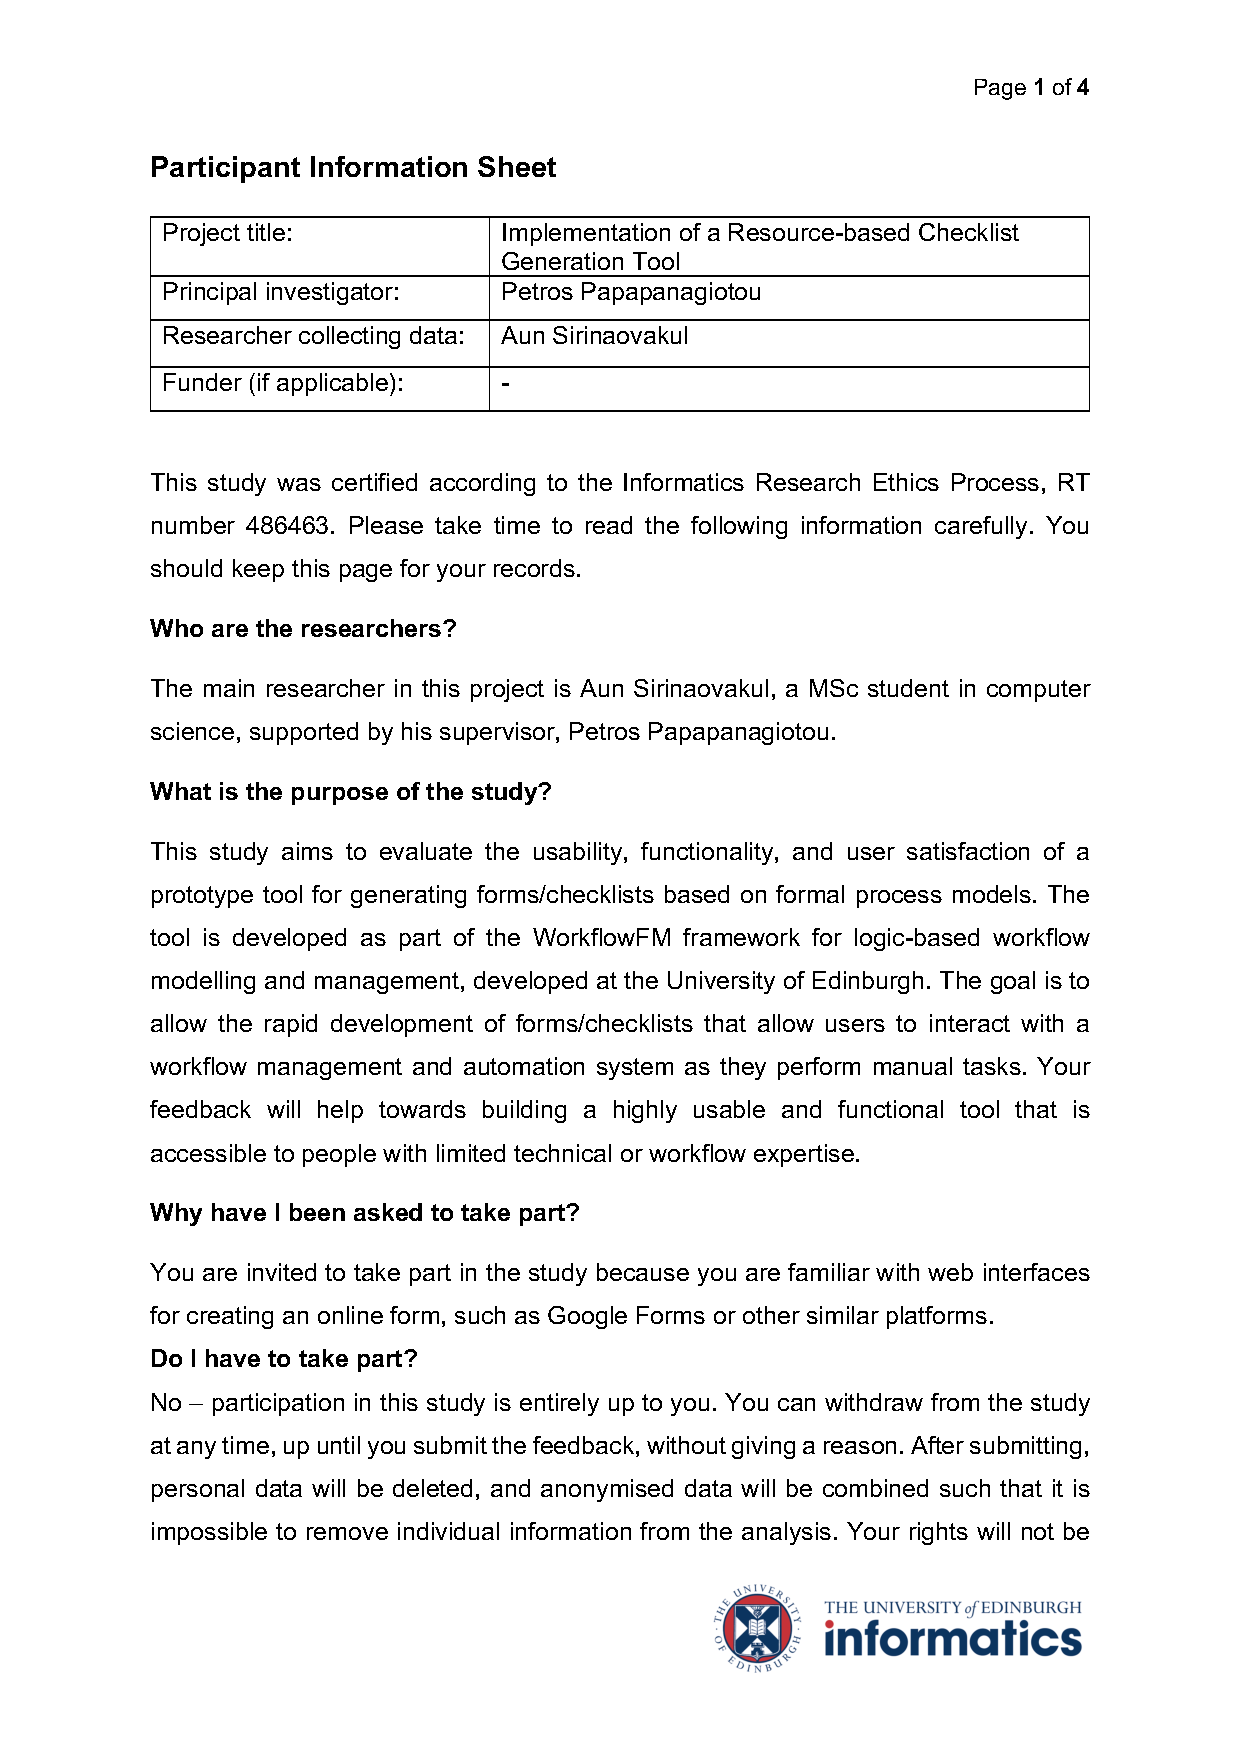
\includepdf[pages=-]{./pdf/PIS.pdf}

\chapter{Participants' consent form}
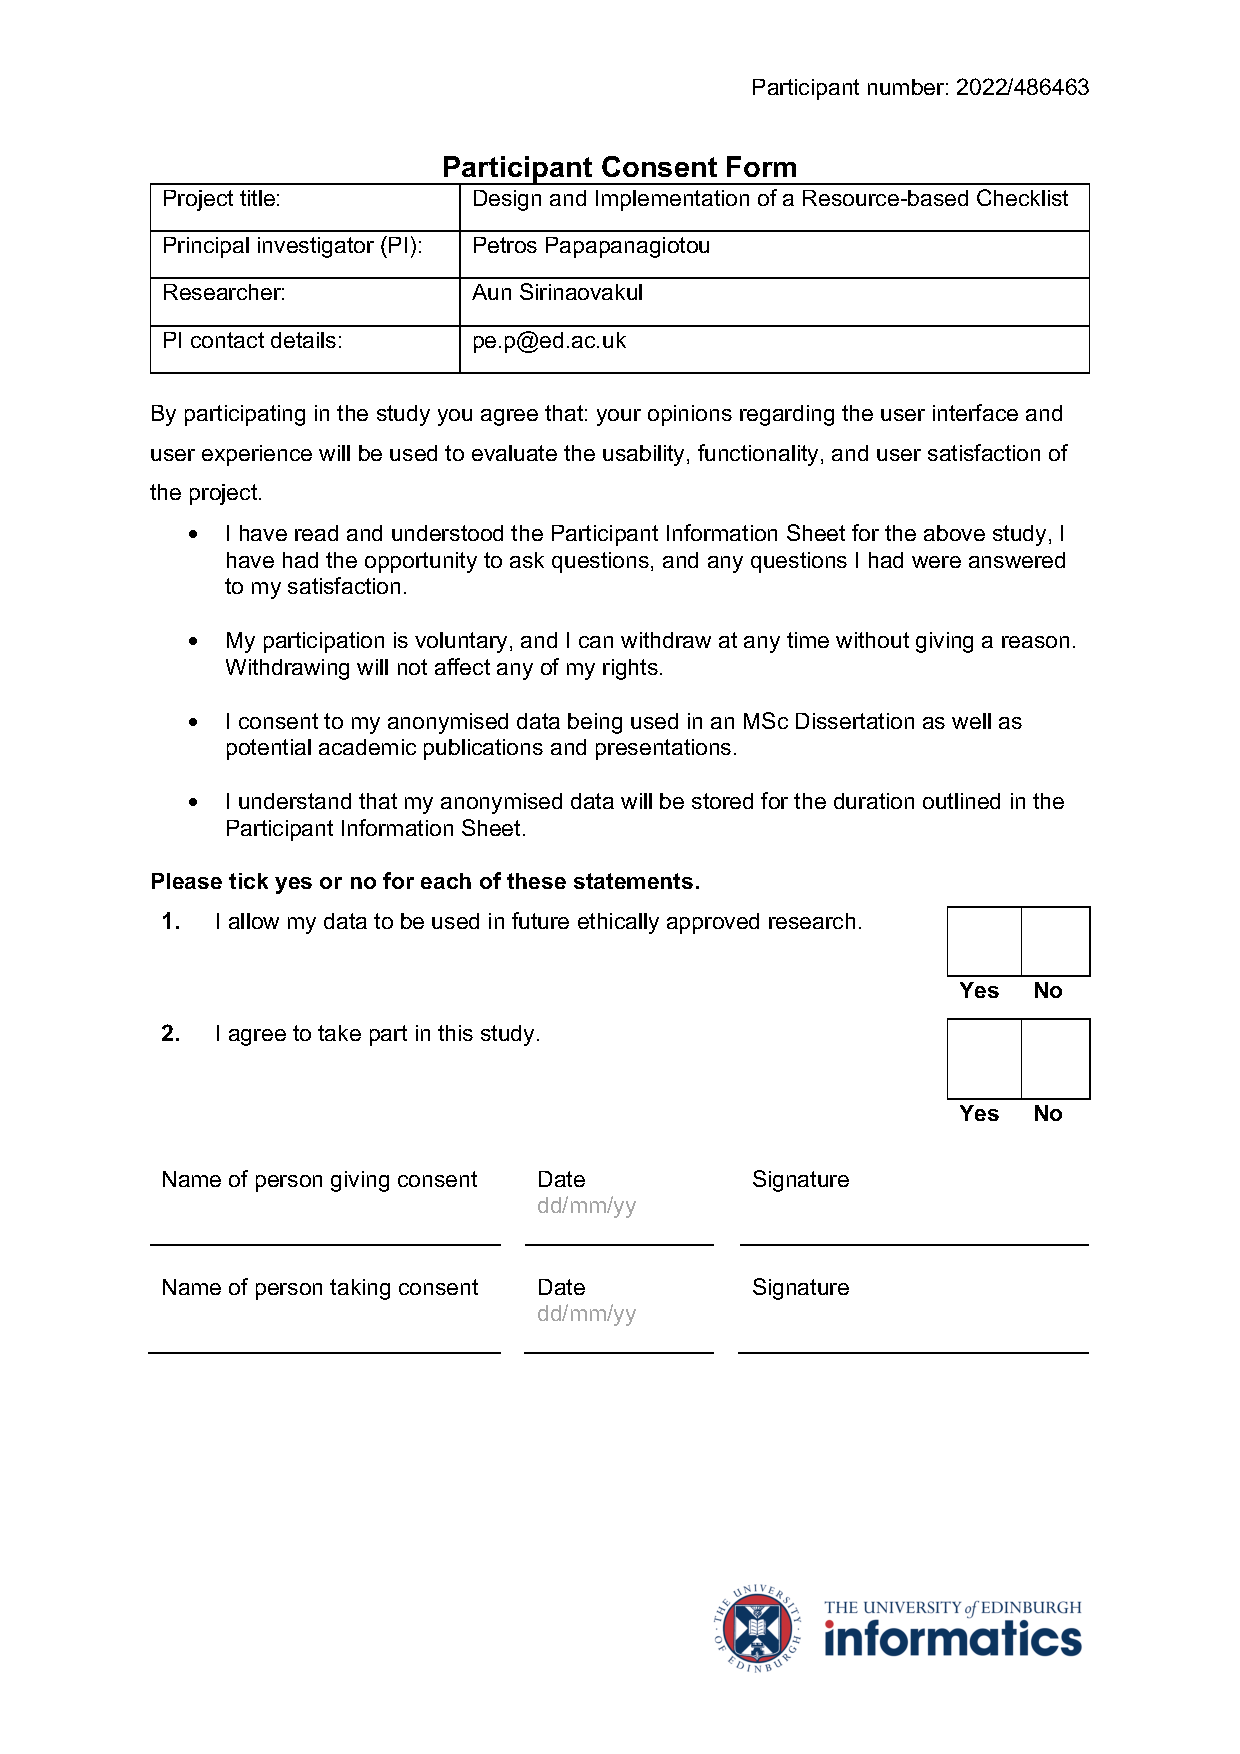
\includepdf[pages=-]{./pdf/Consent Form.pdf}

\chapter{Tasks}

\chapter{Questionaire}


\end{document}
